\documentclass[11pt,a4paper]{report} 

% Für doppelseitigen Ausdruck (nur bei > 60 Seiten sinnvoll)
% \usepackage{ifthen}
% \setboolean{@twoside}{true}
% \setboolean{@openright}{true} 
%Wahrscheinlich eher nicht

% Deutsch
\usepackage[german]{babel} % deutsch und deutsche Rechtschreibung
\usepackage[utf8]{inputenc} % Unicode Text 
\usepackage[T1]{fontenc} % Umlaute und deutsches Trennen
\usepackage{textcomp} % Euro
\usepackage[hyphens]{url}
% statt immer Ab\-schluss\-ar\-beit zu schreiben
% einfach hier sammeln mit -. 
\hyphenation{Ab-schluss-ar-beit}
% Vorsicht bei Umlauten und Bindestrichen
\hyphenation{Ver-st\"ar-ker-aus-gang}
 % eigene Hyphenations, die für das Dokument gelten
\usepackage{amssymb} % Symbole
\usepackage{emptypage} % Wirklich leer bei leeren Seiten

%% Fonts, je ein kompletter Satz an Optionen

% Times New Roman, gewohnter Font, ok tt und serifenlos
%\usepackage{mathptmx} 
%\usepackage[scaled=.95]{helvet}
%\usepackage{courier}

% Palatino mit guten Fonts für tt und serifenlos
\usepackage{mathpazo} % Palatino, mal was anderes
\usepackage[scaled=.95]{helvet}
\usepackage{courier}

% New Century Schoolbook sieht auch nett aus (macht auch tt und serifenlos)
%\usepackage{newcent}

% Oder default serifenlos mit Helvetica 
% ich kann es nicht mehr sehen ...
%\renewcommand{\familydefault}{\sfdefault}

% ein bisschen eine bessere Verteilung der Buchstaben...
\usepackage{microtype}

% Bilder und Listings
\usepackage{graphicx} % wir wollen Bilder einfügen
\usepackage{subfig} % Teilbilder
\usepackage{wrapfig} % vielleicht doch besser vermeiden
\usepackage{listings} % schöne Quellcode-Listings
% ein paar Einstellungen für akzeptable Listings
\lstset{basicstyle=\ttfamily, columns=[l]flexible, mathescape=true, showstringspaces=false, numbers=left, numberstyle=\tiny}
\lstset{language=python} % und nur schöne Programmiersprachen ;-)
% und eine eigene Umgebung für Listings
\usepackage{float}
\newfloat{listing}{htbp}{scl}[chapter]
\floatname{listing}{Listing}

% Seitenlayout
\usepackage[paper=a4paper,width=14.2cm,left=36mm,height=22cm]{geometry}
\usepackage{setspace}
\linespread{1.15}
\setlength{\parskip}{0.5em}
\setlength{\parindent}{0em} % im Deutschen Einrückung nicht üblich, leider

% Seitenmarkierungen 
\newcommand{\phv}{\fontfamily{phv}\fontseries{m}\fontsize{9}{11}\selectfont}
\usepackage{fancyhdr} % Schickere Header und Footer
\pagestyle{fancy}
\renewcommand{\chaptermark}[1]{\markboth{#1}{}}
%\fancyhead[L]{\phv \leftmark}
\fancyhead[RE,LO]{\phv \nouppercase{\leftmark}}
\fancyhead[LE,RO]{\phv \thepage}
% Unten besser auf alles Verzichten
%\fancyfoot[L]{\textsf{\small \kurztitel}}
\fancyfoot[C]{\ } % keine Seitenzahl unten
%\fancyfoot[R]{\textsf{\small Technische Informatik}}

% Theorem-Umgebungen
\newtheorem{definition}{Definition}[chapter]
\newtheorem{satz}{Satz}[chapter]
\newtheorem{lemma}[satz]{Lemma} % gleicher Zähler wie Satz
\newtheorem{theorem}{Theorem}[chapter]
\newenvironment{beweis}[1][Beweis]{\begin{trivlist}
\item[\hskip \labelsep {\textit{#1 }}]}{\end{trivlist}}
\newcommand{\qed}{\hfill \ensuremath{\square}}

% Quellen teilen
\usepackage{bibtopic} 

% Hochschule Logo, noch nicht perfekt
\usepackage{hsmalogo}

% Spezialpakete
\usepackage{epigraph}
\setlength{\epigraphrule}{0pt} % kein Trennstrich

% damit wir nicht so viel tippen müssen, nur für Demo 
\usepackage{blindtext} 

% Zum Zeigen von Fehlern
\usepackage{soul}
\newcommand*\falsch{\st}

\graphicspath{{./images/}}


\usepackage{longtable}
 % alle Pakete und Einstellungen

% Hier anpassen 
\newcommand{\welchethesis}{Bachelor}
\newcommand{\thesisofwas}{of Science}
\newcommand{\studiengang}{Technische Informatik}
\newcommand{\titel}{Entwicklung des Softwaretools ,,Anforderungen und Testen'' für das Anforderungs- und Testmanagement im Softwareentwicklungsumfeld}
\newcommand{\kurztitel}{Arbeitstitel: Anforderungen und Testen}
\newcommand{\autor}{Florian Brunotte}
\newcommand{\datum}{01.02.2021} % Abgabedatum
\newcommand{\ort}{Mannheim}
\newcommand{\referent}{Prof.\ Dr.\ Mark Hastenteufel}
\newcommand{\korreferent}{Prof.\ Dr.\ Martin Damm}

\begin{document}

\begin{titlepage}
  % Kopf der Seite
  \hsmalogo[1] \hfill
  \parbox[b]{60mm}{
    % \textsf würde das Aussehen der ersten Seite ruinieren, 
    % wer will, soll das selbst außen rum machen...
    Fakultät Informationstechnik\\
    Studiengang \studiengang}
  \begin{center}
    % rumfiddeln, damit es für 4 Zeilen gerade noch so geht...
    \rule{1\textwidth}{1pt}\\[-3mm]
    \parbox[t][64mm]{110mm}{% 11 cm für Breite 13, ca. 7 für Höhe 6
      \begin{center}
        \Large{\welchethesis arbeit}\\[2mm]
        {\begin{spacing}{1.13} \huge \bfseries \titel \end{spacing}}
        \vfill
        \Large{\autor} \\[1mm] % keep space to window
        \ 
      \end{center}
    }
    \rule{\textwidth}{1pt}    
    \vfill    
    {\Large Abschlussarbeit} \\[5mm]
    {\large zur Erlangung des akademischen Grades} \\[5mm]
    {\large \welchethesis\ \thesisofwas} \\[5mm]
    \vfill    
    \begin{tabular}{ll} % Mitte der Seite
      Vorgelegt von & \autor \\
      am & \datum \\
      Referent & \referent \\
      Korreferent & \korreferent
    \end{tabular}    
    \vfill
  \end{center}
\end{titlepage}
\cleardoublepage


% Erklärung gemäß der Prüfungsordnung
\thispagestyle{empty}
\subsection*{Schriftliche Versicherung laut Studien- und Prüfungsordnung}

Hiermit erkläre ich, dass ich die vorliegende Arbeit selbstständig verfasst
und keine anderen als die angegebenen Quellen und Hilfsmittel benutzt habe.

\vspace{6em}
\noindent\begin{tabular}{p{0.37\textwidth}p{0.56\textwidth}}
\ort, \datum  & \rule{0.56\textwidth}{0.5pt}\\
              & \makebox[1cm]{\ } \autor
\end{tabular}

\vfill

\cleardoublepage

 % Titelseite, Erklärungen, etc.

\begin{abstract} 

Das Ziel dieser Bachelorarbeit ist die Entwicklung eines leichtgewichtigen \textit{Softwaretools} für das \textit{Anforderungs- und Testmanagement} im \textit{Softwareentwicklungsumfeld}. Dafür gibt es zwar professionelle Tools, diese sind jedoch für Lehrzwecke zu komplex. Diese Lücke soll durch das Ergebnis dieser Bachelorarbeit gefüllt werden mit dem Tool \textit{"`Anforderungen und Testen"'}. Eingesetzt werden kann diese Anwendung im Rahmen von kleinen Semesterprojekten, die dadurch unterstützt werden sollen, ohne vom Wesentlichen abzulenken.

Geschrieben wurde das Tool als \textit{Webanwendung} in der Programmiersprache \textit{Python} und mit dem \textit{Webframework Django}.
Ergänzend dazu wurde auch \textit{HTML}, \textit{CSS} und \textit{JavaScript} verwendet. Durch einen \textit{UI-Prototypen} konnte das generelle Aussehen der Anwendung getestet werden. Dadurch konnten bereits Rückmeldungen für die Implementierung erhalten werden.

Der Fokus liegt dabei auf der Erstellung von simplen und leicht verständlichen Benutzerschnittstellen, welche durch einen \textit{Usabilitytest} auf ihre Benutzerfreundlichkeit überprüft werden. Daneben soll das \textit{Softwaretool} auch über eine Datenbankanbindung verfügen, zum Beispiel an \textit{PostgreSQL}. Aus diesem Grund spielt das Datenbankdesign ebenfalls eine wichtige Rolle in dieser Arbeit.


\end{abstract}

\tableofcontents %Inhaltsverzeichnis wird erstellt

\chapter{Grundlagen} 
\label{c:grund}

Es soll ein leichtgewichtiges \textit{Softwaretool} entwickelt werden, welches die Lehrveranstaltung unterstützt. Das \textit{Tool} sollte sich auf die Kernfunktionalitäten beschränken, damit sich die Anwender auf das Wesentliche konzentrieren können. Andere \textit{Softwaretools}, die auf dem Markt verfügbar sind, sind für den Einsatz in der Lehre nicht geeignet, da sie nicht nur zu komplex sind, sondern auch zu große Kosten mit sich bringen. Eine intuitive und simple Software, wie \textit{"`Anforderungen und Testen"'} soll hier Abhilfe schaffen.

Im Nachfolgenden wird das \textit{Anforderungs- und Testmanagement} erklärt. Danach werden die professionellen Tools vorgestellt, an denen sich die Software  \textit{"`Anforderungen und Testen"'} orientiert, bevor zuletzt das Thema \textit{Usability} angesprochen wird.

\section{Anforderungs- und Testmanagement} 
\label{s:anfundtest}

Im Rahmen des \textit{Anforderungsmanagement} gibt es verschiedene Arten von Anforderungen, die bei der Entwicklung eines Systems erfasst werden sollten. Es gibt die \textit{Produkt-} beziehungsweise \textit{Stakeholderanforderungen}, die aus der Kunden- oder Nutzersicht entstehen. Damit werden die zu erreichenden Ziele und der Zweck des Systems beschrieben, die die \textit{Stakeholder} verfolgen \cite{htm}. 

Als \textit{Stakeholder} werden Individuen, Gruppen oder Organisationen bezeichnet, die von einem Projekt beeinflusst werden, das Projekt beeinflussen oder durch das Ergebnis des Projekts beeinflusst werden \cite{pmbok}. Beispiele für \textit{Stakeholder} sind die Kunden oder Geschäftspartner in einem Projekt. In diesem Projekt ist Herr Prof. Dr. Hastenteufel ein Stakeholder.


Daraufhin werden basierend auf den Anforderungen der \textit{Stakeholder} \textit{Software-Anforderungen} aufgestellt. Diese müssen von der Software erfüllt werden, damit der Kunde ein System erhält, das seinen Vorstellungen entspricht \cite{htm}. Zur Überprüfung der Funktionalitäten der Software werden Tests geschrieben und durchgeführt. Die \textit{Stakeholder} werden auf diesem Weg über die Qualität der Software informiert \cite{powerpoint}.


\section{Marktverfügbare Tools} 
\label{chap:Tools}


Es gibt verschiedene Tools mit diversen Gründen, die einen Ausschluss von der Benutzung in einer Lehrveranstaltung rechtfertigen. Sie können andere, eigene Begriffe verwenden, hohe Kosten nach sich ziehen oder zu komplex sein. Das Ziel der Lehrveranstaltung sollte das \textit{Anforderungs- und Testmanagement} sein und nicht das Kennenlernen neuer Tools. Diese sollten die Lehrveranstaltung nur unterstützen und nicht dominieren. Das Tool sollte also möglichst selbsterklärend sein, sodass das Gelernte im Unterricht sofort angewendet werden kann. Zu den verschiedenen Tools, die es auf dem Markt gibt, werden an dieser Stelle die Aspekte präsentiert, die die Tools ungeeignet machen für den Einsatz in Semesterveranstaltungen. Daneben werden aber auch die Aspekte präsentiert, an denen sich die erstellte Software orientiert hat.











%1. Tool testcollab

\begin{figure}[htpb]
  \centering
  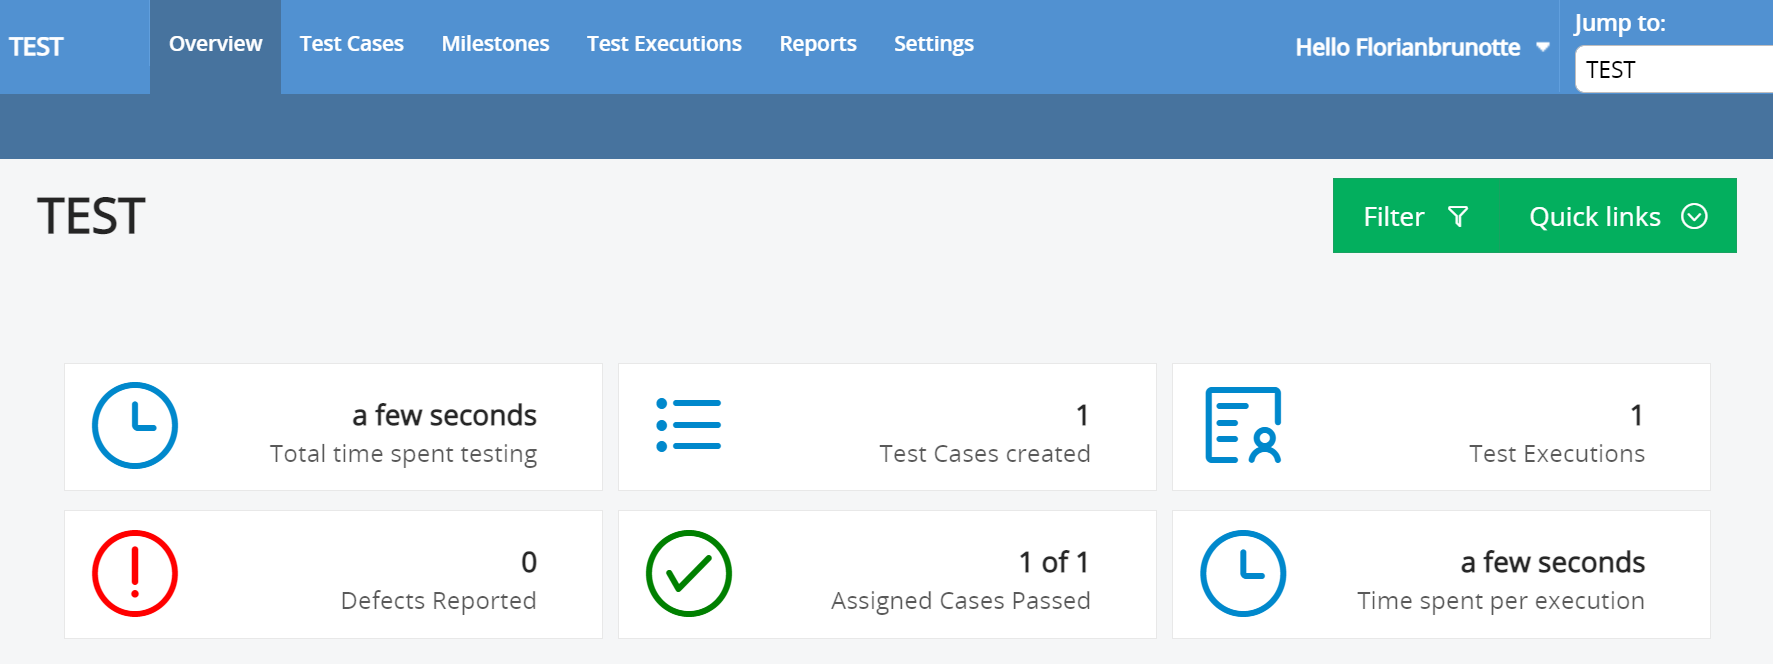
\includegraphics[width=1\textwidth]{testcollab_dash1.png}
  \caption{Das Dashboard in Testcollab, aus \cite{testcollab}}
  \label{f:testcollab-dash}
\end{figure}

\begin{figure}[htpb]
  \centering
  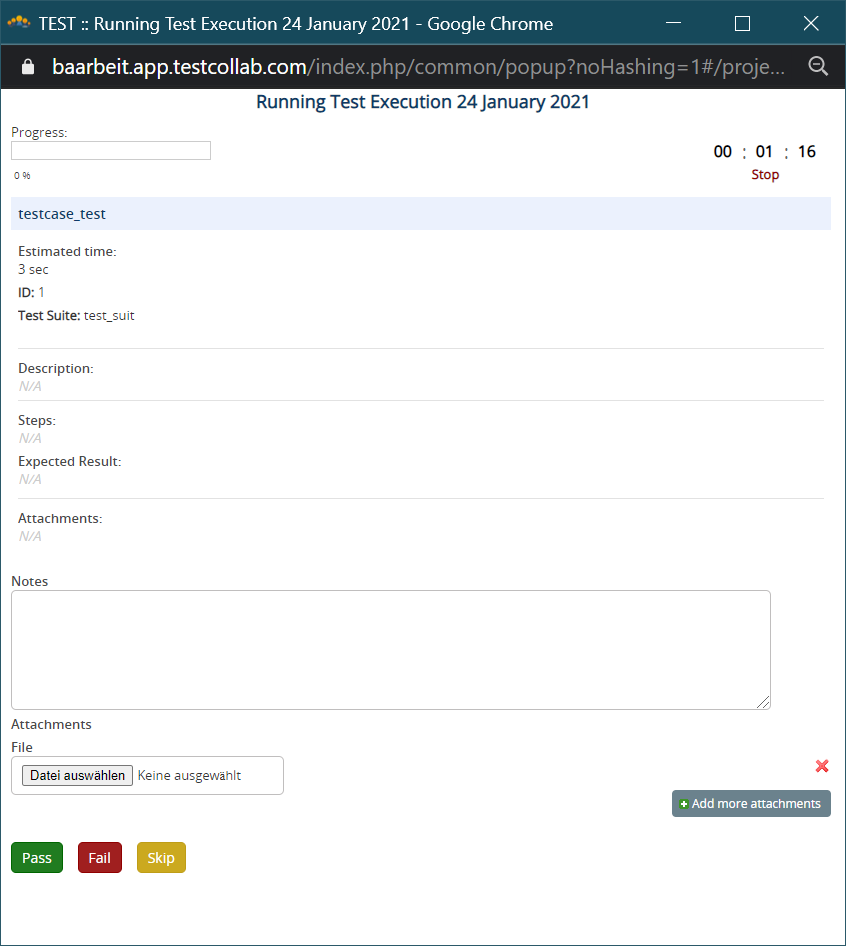
\includegraphics[width=1\textwidth]{testcollab_run.png}
  \caption{Die Testrun Druchführung in Testcollab, aus \cite{testcollab}}
  \label{f:testcollab-testrun}
\end{figure}

\begin{figure}[htpb]
  \centering
  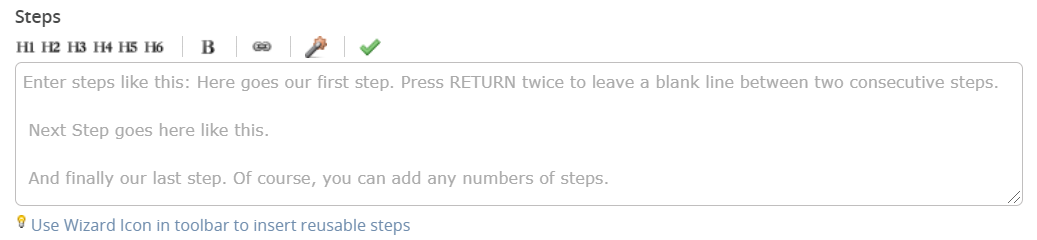
\includegraphics[width=1\textwidth]{testcollab_steps.png}
  \caption{Die Eingabe von Testschritten in Testcollab, aus \cite{testcollab}}
  \label{f:testcollab-testschritt}
\end{figure}

Das erste Tool, das an dieser Stelle vorgestellt werden soll, ist \textit{Testcollab} \cite{testcollab}. Dieses Tool ist das einzige, dass eine kostenlose Version anbietet. Bei der kostenlose Variante können maximal drei Personen gleichzeitig an einem Projekt arbeiten, was im Semester eventuell zu einem Problem führen könnte, dass es somit zu viele Gruppen gibt \cite{testcollabprice}. Daneben gibt es noch die Limitierung, dass in einem Projekt nur maximal 200 \textit{Testcases} und 300 \textit{Testruns} erstellt werden können. Da es sich im Semester nur um kleine Projekte handeln wird, sollte diese Limitierung kein Problem darstellen.


Aus Sicht der Benutzerfreundlichkeit fällt bei der Eingabe der \textit{Testschritte} auf, dass diese mit Leerzeilen dazwischen eingegeben werden sollen, wie in der Abbildung \ref{f:testcollab-testschritt} präsentiert. Die Eingabe der Leerzeile könnte vergessen werden, dadurch wären statt vieler \textit{Testschritte} nur ein großer \textit{Testschritt} definiert. Sinnvoller wäre eine Implementierung, in der jeder \textit{Testschritt} ein eigenes Feld hat, zum Beispiel bei der Implementierung als Tabelle. Das Design der \textit{Testrunseite}, die in der Abbildung \ref{f:testcollab-testrun} zu sehen ist, könnte allerdings übernommen werden.

Ein Nachteil des Tools ist, dass es keine Aussage darüber macht bei welchem Schritt der \textit{Testrun} durchgefallen ist. Es gibt nur eine Aussage darüber, ob die gesamte \textit{Test Suite} erfolgreich war oder nicht.



Andererseits wurde aus dem \textit{Dashboard}, das in der Abbildung \ref{f:testcollab-dash} dargestellt ist, die Navigationsleiste am oberen Bildschirmrand übernommen, damit die Nutzer immer einen Überblick haben, an welcher Stelle sie sich gerade befinden. Gleichzeitig wurde die Begrüßung oben rechts auch übernommen, dadurch soll der erfolgreiche \textit{Login} signalisiert werden. Ebenfalls gibt es in dem \textit{Dashboard} ein Ausrufezeichen, wenn etwas fehlgeschlagen ist. Dadurch könnte die Aufmerksamkeit der Nutzer direkt auf die wichtigsten Probleme im Projekt gelenkt werden.
























%2. Tool Jira Xray

\begin{figure}[htpb]
  \centering
  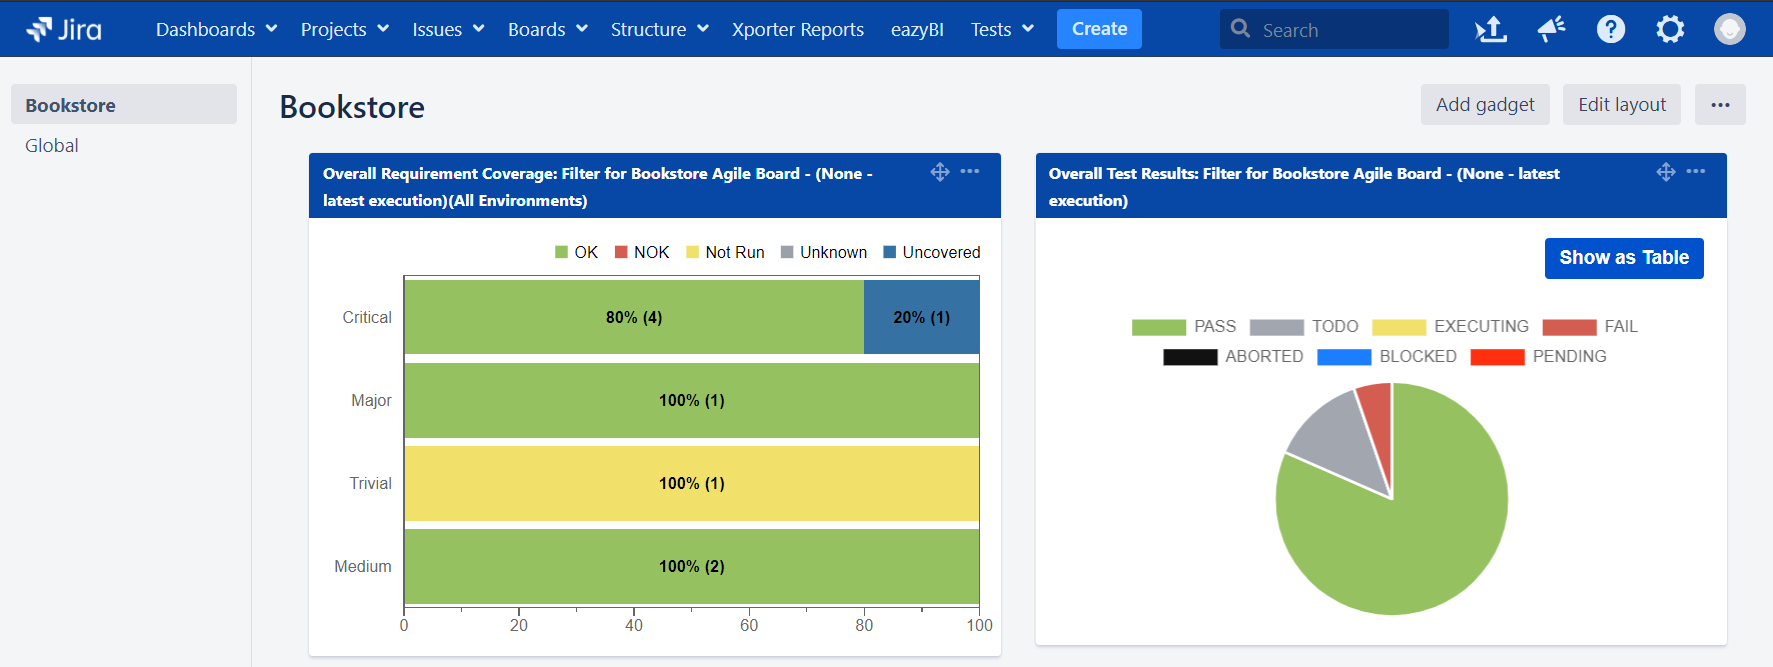
\includegraphics[width=1\textwidth]{jira_dash.png}
  \caption{Das Dashboard in Jira, aus \cite{xray}}
  \label{f:jiradash}
\end{figure}


\begin{figure}[htpb]
  \centering
  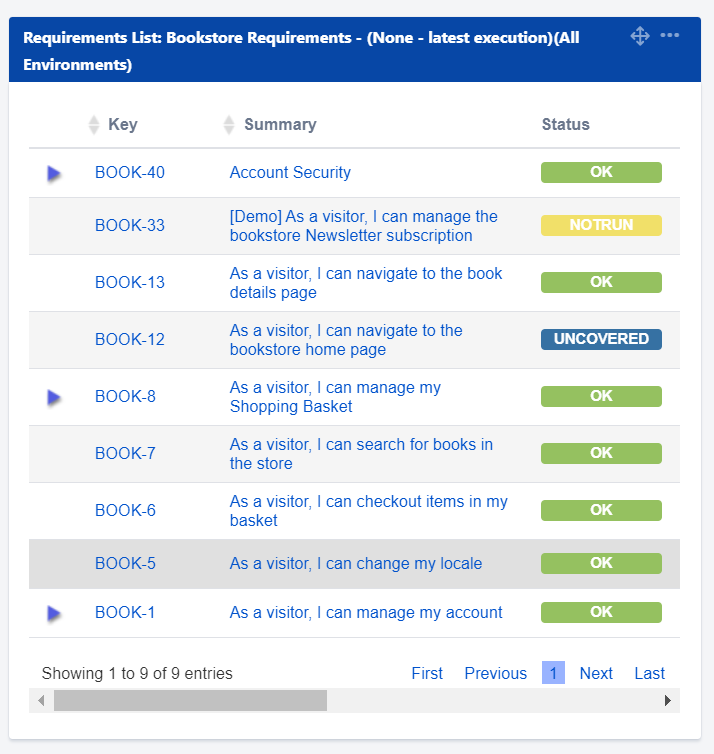
\includegraphics[width=1\textwidth]{jira_dash2.png}
  \caption{Die Requirements Liste in Jira, aus \cite{xray}}
  \label{f:jiradash2}
\end{figure}


Das nächste Tool ist \textit{Xray} \cite{xray}. Es ist eine Erweiterung des Tools \textit{Jira}, welches für \textit{agiles Projektmanagement} verwendet wird \cite{jiraxray}. Auf den ersten Blick wirkt das Tool zu komplex, als das es eine Lehrveranstaltung unterstützend begleiten kann.

Die Visualisierung der Daten durch Kuchendiagramme auf dem \textit{Dashbaord}, wie in der Abbildung \ref{f:jiradash} gesehen werden kann, könnte übernommen werden. Durch die Farben können die Nutzer sofort sehen, ob es ein Problem im Projekt gibt. Bei der Liste der \textit{Requirements}, die in der Darstellung \ref{f:jiradash2} abgebildet ist, kann der Status abgelesen werden. Auf diesem Weg können die Nutzer auch anhand der Farben erkennen, welche Elemente noch Aufmerksamkeit benötigen.







%3. Tool testlodge

\begin{figure}[htpb]
  \centering
  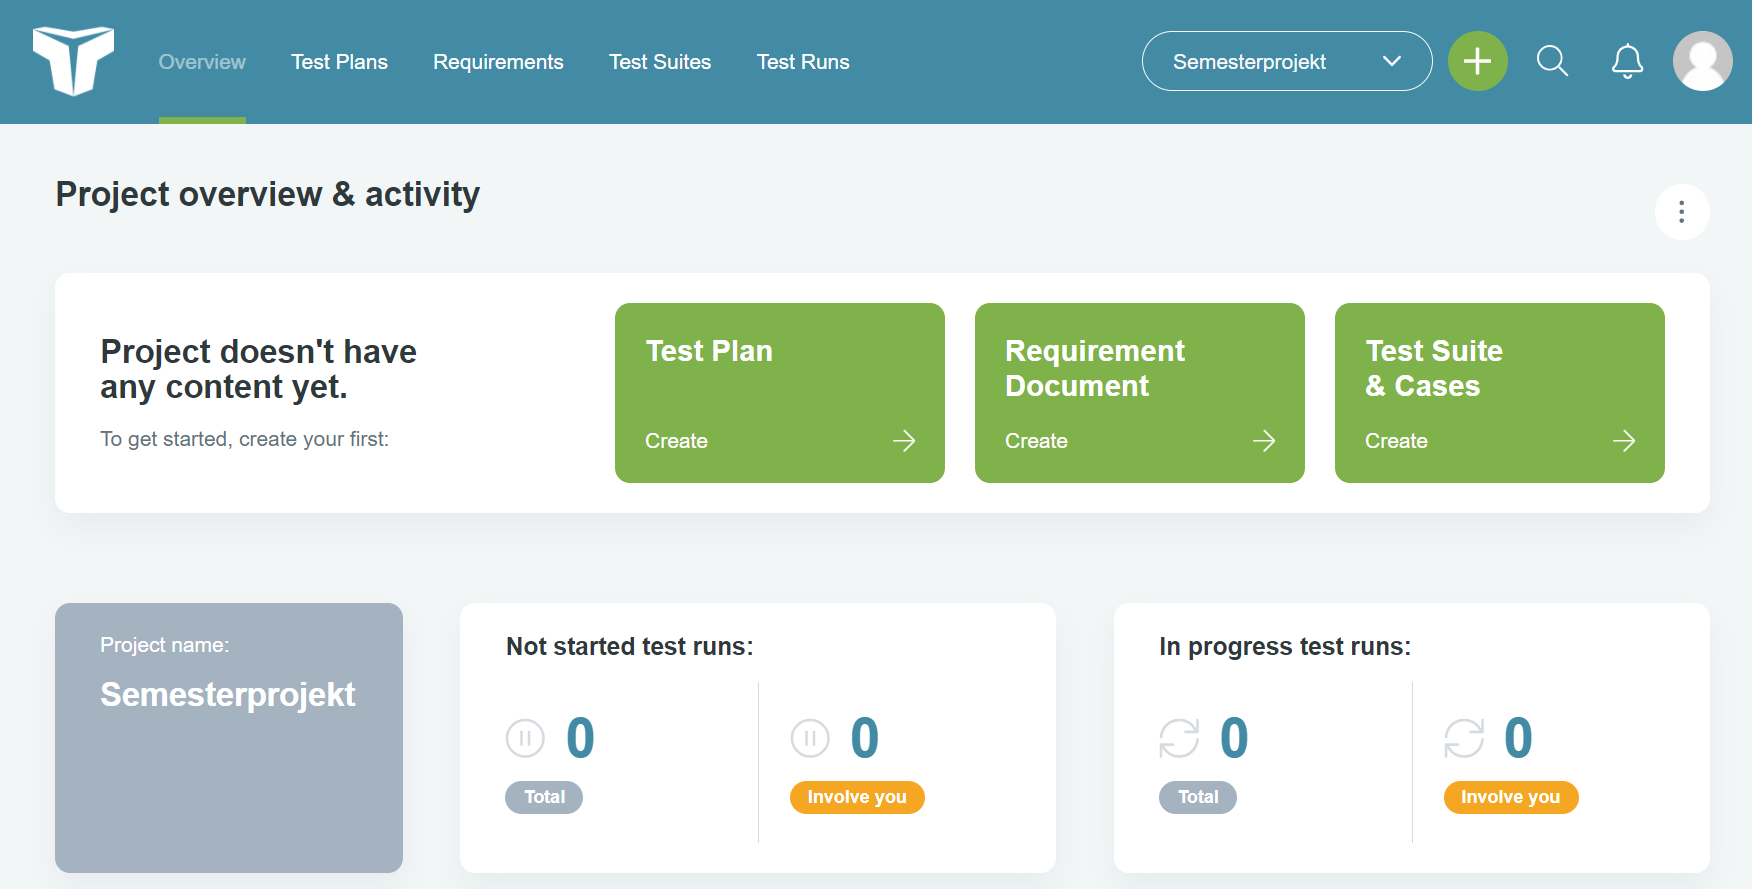
\includegraphics[width=1\textwidth]{lodgedash.png}
  \caption{Das Dashboard von Testlodge, aus \cite{testlodge}}
  \label{f:lodgedash}
\end{figure}


Beim Tool \textit{Testlodge} muss vor dem Erstellen von \textit{Requirements} ein \textit{Requirement Document} erstellt werden und vor dem Erstellen von \textit{Testcases} eine \textit{Test Suite} \cite{testlodge}. Darin werden dann die jeweiligen Elemente gesammelt. Diese Option entfällt bei dem Tool \textit{"`Anforderungen und Testen"'}. Es sollte sofort eine Möglichkeit geben neue Elemente zu erstellen, ohne über den Umweg einer weiteren Ebene gehen zu müssen.

Es sollte die Unterscheidung zwischen \textit{Requirements}, \textit{Testcases} und \textit{Testruns} übernommen werden, damit die Nutzer besser unterscheiden können, was gerade bearbeitet wird. Diese Unterscheidung gab es nur in diesem Tool und kann in der Menüleiste in der Graphik \ref{f:lodgedash} gesehen werden.

\textit{Testlodge} bietet auch die Möglichkeiten an, \textit{Testruns} an andere Leute im Projekt anzuweisen. Das ist ein weiteres Feature, das aufgegeben wird, um sich auf das Wesentliche zu begrenzen. Das Aussehen der Software \textit{"`Anforderungen und Testen"'} wird, aufgrund der Aufteilung der Elemente, am meisten von diesem Tool beeinflusst.



















% 4. Tool testcaselab


\begin{figure}[htpb]
  \centering
  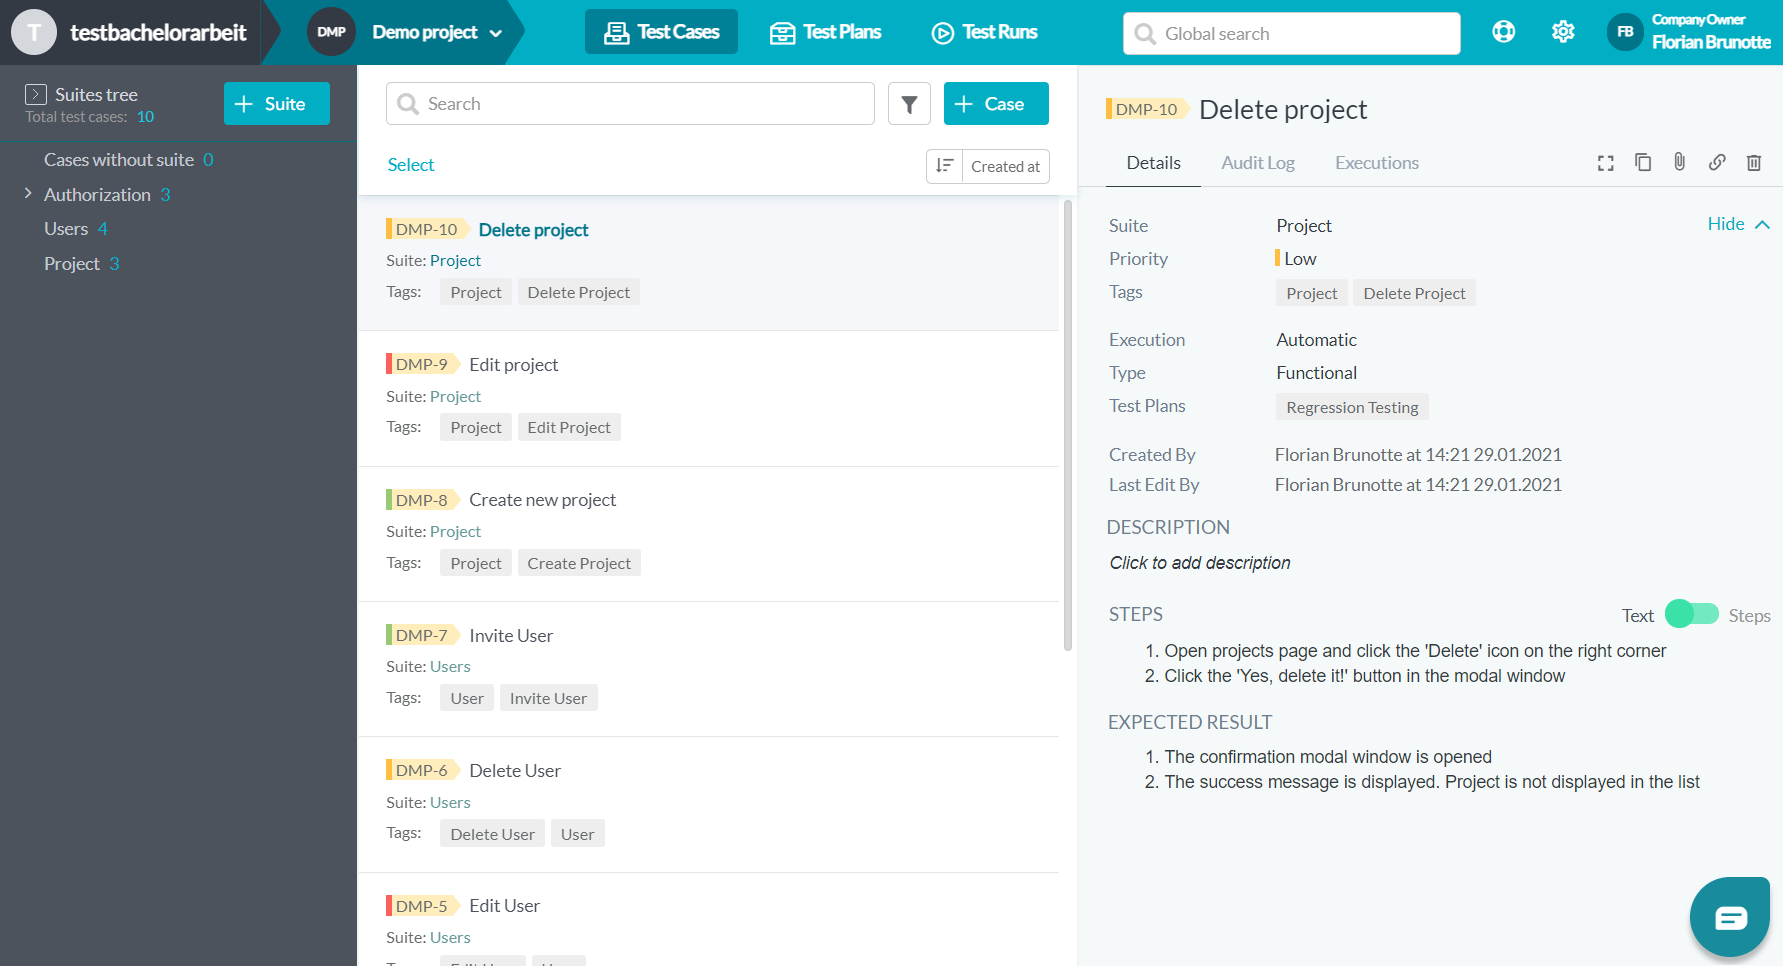
\includegraphics[width=1\textwidth]{testcaselabdash.png}
  \caption{Das Dashboard von Testcaselab, aus \cite{testcaselab}}
  \label{f:testcaselabdash}
\end{figure}

Ein weiteres Tool, welches für das \textit{Anforderungs- und Testmanagement} entwickelt wurde, ist \textit{Testcaselab} \cite{testcaselab}. Inspirierend bei diesem Tool ist die Anzeige der Elemente als Liste auf der linken Seite mit der detaillierten Ansicht auf der rechten Seite. Diese Ansicht kann in der Abbildung \ref{f:testcaselabdash} gesehen werden. 





%5. Tool qatouch



\begin{figure}[htpb]
  \centering
  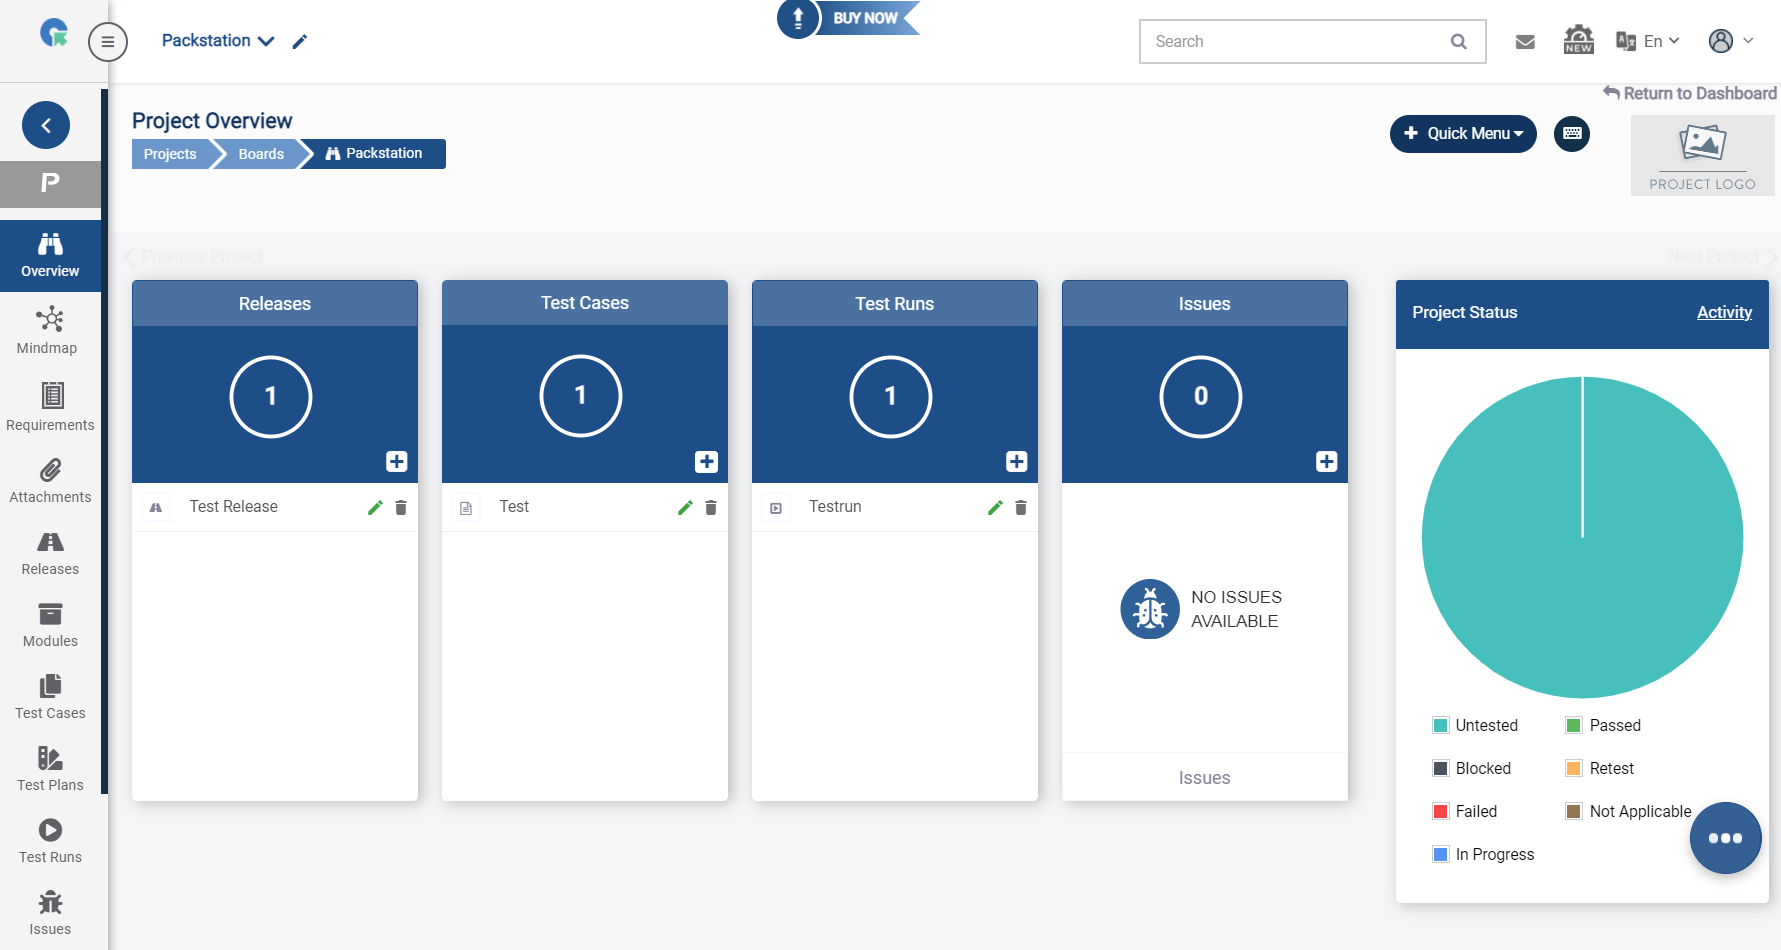
\includegraphics[width=1\textwidth]{qatouch.png}
  \caption{Das Dashboard von QA Touch, aus \cite{qatouch}}
  \label{f:qatouch}
\end{figure}


Das letzte Tool, das an dieser Stelle erwähnt werden soll, ist \textit{QA Touch} \cite{qatouch}. Negativ auffallend bei diesem Tool ist die Navigation der Seite. Die Seite stellt Inhalte häufig mit Pop-up-Fenstern dar, wodurch es schwierig wird sich den jetzigen Standpunkt der Webseite klar zu machen, und das obwohl es eine Leiste gibt, die den Verlauf auf der Seite anzeigt. Diese Leiste kann in der oberen Bildhälfte der Abbildung \ref{f:qatouch} gesehen werden. Durch diese Unübersichtlichkeit ist dieses Tool für eine Benutzung in der Lehrveranstaltung eher ungeeignet.








%Zusammenfassung


\begin{table}[htpb]
\caption{Zusammenfassung der Tools}
\begin{center}
\begin{tabular}{|p{0.2\textwidth}|p{0.4\textwidth}|p{0.4\textwidth}|}
    \hline
    \multicolumn{1}{|c|}{\textbf{Tool}} & 
	\multicolumn{1}{|c|}{\textbf{Pro}}& 
	\multicolumn{1}{|c|}{\textbf{Contra}} \\
    \hline
    Testcollab & kostenlose Variante wird angeboten & Eingabe der Testschritte nicht benutzerfreundlich und keine Aussage, welcher Testschritt fehlgeschlagen ist \\
    \hline
    Xray & Visualisierung macht Probleme sofort ersichtlich & hohe Komplexität und kostenlose Version ist nur als Free Trial verfügbar \\
    \hline
    Testlodge & Unterscheidet zwischen Requirements, Testcases und Testruns & kostenlose Version ist nur als Free Trial verfügbar\\
    \hline
    Testcaselab & Listenansicht der Elemente mit anschließender Detailansicht & kostenlose Version ist nur als Free Trial verfügbar \\
    \hline
    QA Touch & Verlauf der Seite wird angezeigt & ersichtliche Navigation der Seite wird durch Pop-up-Fenster eingeschränkt und kostenlose Version ist nur als Free Trial verfügbar\\
	\hline
	
\end{tabular}
\end{center}
\label{t:zusammenfassung}
\end{table}

In der Tabelle \ref{t:zusammenfassung} sind die vorgestellten Tools mit den Punkten dargestellt, die für und gegen sie sprechen. Ergänzend dazu soll an dieser Stelle noch gesagt werden, dass nur das Tool \textit{Testcollab} eine kostenlose Variante anbietet, die auch zeitlich nicht begrenzt ist. Ein generelles Problem bei allen Tools ist die Tatsache, dass es bei keinem die Möglichkeit gab eine \textit{Traceability-Matrix} zu erzeugen. Wie im späteren Kapitel \ref{c:Anf} gezeigt, wurde so eine Matrix jedoch gefordert.


\section{Usability}

Die \textit{Usability}, beziehungsweise die Gebrauchstauglichkeit, wird beschrieben als
der Nutzungskontext, in dem ein Produkt durch einen Nutzer effektiv, effizient und zufriedenstellend genutzt werden kann. Der Nutzer möchte durch die Benutzung des Produkts ein Ziel erreichen \cite{isousa}. Dahingegen wird ein \textit{User Interface}, beziehungsweise eine Nutzungsschnittstelle, definiert als Bestandteile eines interaktiven Systems, die für den Nutzer nötig sind, um sein Ziel zu erreichen. Dazu stellt das User Interface Informationen und Steuerelemente zur Verfügung \cite{isoui}.

Eine Übersicht guter Praktiken beim Design von \textit{User Interfaces} bieten dabei die \textit{zehn Usability-Heuristiken nach Nielsen}. Diese sind in der Tabelle \ref{t:ui} zusammengetragen.

\begin{table}[htpb]
\caption{Die zehn Usability-Heuristiken nach Nielsen, aus \cite{nielsend} und \cite{nielsen}}
\begin{center}
\begin{tabular}{|p{0.3\textwidth}|p{0.7\textwidth}|}
    \hline
    \multicolumn{1}{|c|}{\textbf{Datei}} & 
	\multicolumn{1}{|c|}{\textbf{Inhalt}} \\
    \hline
    1. Sichtbarkeit des Systemstatus & Die Nutzer sollten eine Rückmeldung bekommen zu ihren Interaktionen mit dem System. Darüber hinaus sollten sie auch wissen an welchem Punkt sie sich in einer Aktion befinden.\\
	\hline
  2. Übereinstimmung von System und realer Welt & Das System sollte Begriffe verwenden, die der Kunde aus der realen Welt erwarten würde.\\
    \hline
   3.  Nutzerkontrolle und -freiheit & Falls Nutzer einen Fehler machen, sollten sie die Möglichkeit haben diesen Fehler zu korrigieren oder sogar den aktuellen Prozess abzubrechen	\\
    \hline
    4. Konsistenz und Standards & Nutzer sollten nicht überlegen müssen, ob verschiedene in der Software verwendete Begriffe vielleicht doch das gleiche bedeuten. Stattdessen sollten die gleichen Begriffe für die gleichen Funktionen benutzt werden.\\
    \hline
   5. Fehlervermeidung & Es sollte vermieden werden, dass Nutzer fehlerhafte Eingaben tätigen können. Das System sollte generell Fehler vermeiden. \\
   \hline
   6. Erkennen anstatt Erinnern & Nutzer sollten die Software benutzen können ohne sich an Dialoge erinnern zu müssen \\
    \hline
  7. Flexibilität und effiziente Nutzung & Abkürzungen sollten erfahrenen Nutzern eine effiziente Bedienung ermöglichen. Unerfahrene Nutzer sollten durch Anleitungen angelernt werden. \\
    \hline
   8. Ästhetisches und minimalistisches Design & Der Inhalt eines UI sollte auf das Wesentliche reduziert werden. \\
    \hline
   9. Hilfe bei Fehlern & Fehlermeldungen sollten das Problem konkret beschreiben und eine konstruktive Lösung vorschlagen. Außerdem sollten sie in leicht verständlicher Sprache geschrieben sein. \\
    \hline
    10. Hilfe und Dokumentation & Soweit möglich, sollten Nutzer ohne Hilfe die Software bedienen können. Falls nötig sollte sie aber bereitstehen.\\
   
    \hline
\end{tabular}
\end{center}
\label{t:ui}
\end{table}



\chapter{Planung} \label{chap:Anforderungen}
Vor der Implementierung der Anwendung sollte geklärt sein, welche Anforderungen, wie realisiert werden sollen. Basierend auf den vorgegebenen Anforderungen wurden \textit{UML-Diagramme} erstellt. Darüber hinaus wurden sowohl ein \textit{Entity-Relationship Diagramm} erstellt, mit dem das Datenbankdesign beschrieben wird, als auch ein \textit{UI-Prototyp} vorgestellt, mit dem die Navigation und das Aussehen der Seite getestet werden kann.


\section{Anforderungsanalyse} \label{c:Anf}


Die Anforderungen an die Software wurden von Herrn Prof. Dr. Hastenteufel in Form eines Anforderungsdokuments erhoben. Darin enthalten sind die folgenden Nutzerrollen: 

\begin{itemize}
\setlength\itemsep{0.1em}
\item Admin

\item Professor

\item Student beziehungsweise Entwickler und/oder Tester

\item Nutzer (umfasst alle Rollen)

\end{itemize}


\begin{table}[htpb]
\caption{Funktionsblock Administration}
\begin{center}
\begin{tabular}{|p{0.1\textwidth}|p{0.9\textwidth}|}
    \hline
    \multicolumn{2}{|c|}{Administration}\\
    \hline
    A10 & Als Nutzer will ich mich einloggen können und einen 				persönlichen Startbildschirm mit meinen
	Projekten sehen
	(Bemerkung: Im optimalen Fall SSO mit SWT / HS Account)\\
	\hline
    A20 & Als Admin will ich neue Projekte erstellen können\\
    \hline
    A30 & Als Admin will ich Studenten zu Projekten zuordnen können		\\
    \hline
\end{tabular}
\end{center}
\label{t:funkadmin}
\end{table}


\begin{table}[htpb]
\caption{Funktionsblock Statistiken}
\begin{center}
\begin{tabular}{|p{0.1\textwidth}|p{0.9\textwidth}|}

    \hline
    \multicolumn{2}{|c|}{Statistiken}\\
    \hline
    A40 &  Als Professor will ich Statistiken zu den einzelnen Projekten sehen.
(Bemerkung: Statistiken sind genauer zu definieren) Das können z.B. sein    
\begin{itemize}
\setlength\itemsep{0.1em}
\item Anzahl der Anforderungen pro Projekt
\item Anzahl der Testfälle pro Projekt
\item Anzahl der durchgeführten Testruns pro Projekt
\item Für jede Anforderung die zugehörigen Testfälle (Testfallabdeckung)
\item Für jede Anforderung den Status der zugehörigen Testruns (Testabdeckung)
\item Für jeden Testfall die damit abgedeckten Anforderungen
\item Für jeden Testfall den Status der zugehörigen Testruns
\item Angaben über die mit der Testfalldurchführung verbrachte Zeit (minimal, maximal, Durchschnitt, Summe)
\item Ein übersichtliches Dashboard des Projektstatus (Klärungsbedarf)
\item Für jedes Teammitglied die Anzahl der Anforderung/Testfälle/Testruns 

\end{itemize}

    \\
\hline
    A50 & Als Student will ich für mein aktuelles Projekt Statistiken sehen\\
    \hline
  
\end{tabular}
\end{center}
\label{t:funkstat}
\end{table}



\begin{table}[htpb]
\caption{Funktionsblock Anforderungs- und Testmanagement}
\begin{center}
\begin{tabular}{|p{0.05\textwidth}|p{0.95\textwidth}|}
  \hline

    \multicolumn{2}{|c|}{Anforderungs- und Testmanagement}\\
    \hline
        A60 &  Als Student will ich Anforderungen spezifizieren können.
Bemerkung: Anforderungen sollten mindestens folgende Attribute enthalten:
\begin{itemize}
\setlength\itemsep{0.1em}
\item Eine Anforderungs-ID (automatisch generiert)
\item Einen Namen
\item Die eigentlichen Anforderungen
\item Kommentar
\item Bearbeiter (automatisch)
\item Datum der initialen Erstellung und letzte Änderung
\item Die damit verbundenen Testfälle
\item Kategorie (Klärungsbedarf)

\end{itemize} \\
\hline
           A70 & Als Student will ich Testfälle spezifizieren können.
Bemerkung: Testfälle enthalten mindestens folgende Attribute:
\begin{itemize}
\setlength\itemsep{0.1em}
\item Eine Testfall-ID (automatisch generiert)
\item Einen Namen
\item Vorbedingungen
\item Den eigentlichen Testfall aufgegliedert in:
\begin{itemize}
\setlength\itemsep{0.1em}
\item Durchzuführende Schritte
\item Erwartetes Ergebnis
\item Tatsächliches Ergebnis (wird bei der Testfalldurchführung ausgefüllt)

\end{itemize}
\item Kommentar
\item Bearbeiter (automatisch)
\item Datum der initialen Erstellung und letzte Änderung
\item Die mit dem Testfall getesteten Anforderungen


\end{itemize} \\


    \hline
       A80 & Als Student will ich Testfälle durchführen können (Testfalldurchführung/Testruns).
Bemerkung: Testfalldurchführungen enthalten mindestens folgende Attribute:
       
       \begin{itemize}
\setlength\itemsep{0.1em}
\item ID des zugrundeliegenden Testfalls
\item Datum des Testruns
\item Kommentarfeld für z.B. Dokumentation der Testumgebung
\item Für jeden Schritt des Testfalls: pass oder fail
\item Für jeden Schritt des Testfalls: Kommentar
\item Gesamtstatus der Testdurchführung: berechnet aus den einzelnen Testschritten
\item Name des durchführenden Testers
\item Potentiell Anhänge für die Testevidenz (png, pdf, …)
\item Dauer der Durchführung in min

\end{itemize}\\
    \hline
    
\end{tabular}
\end{center}
\label{t:funkanfundtest}
\end{table}



Die Anforderungen an die Software sind in drei Funktionsblöcke aufgeteilt, welche in den Tabellen \ref{t:funkadmin}, \ref{t:funkstat} und \ref{t:funkanfundtest} betrachtet werden können. Der Klärungsbedarf, der bei den Inhalten des \textit{Dashboards} vorhanden war, konnte durch den \textit{UI-Prototypen}, der in Kapitel \ref{s:ui} vorgestellt wird, gelöst werden. Zusätzlich wurde die Terminologie vereinbart, dazu wurden die englischen Begriffe ausgewählt. Die Anforderungen werden in der Software \textit{Requirements}, die Testfälle \textit{Testcases} und die Testfalldurchführungen \textit{Testruns} genannt. Alle drei Begriffe werden unter der Bezeichnung \textit{Element} zusammengefasst. Bei der Kategorie der \textit{Requirements}, aus der Anforderung A60, wurde der Klärungsbedarf dadurch gelöst, dass die Kategorien erstmal nur eine Auswahl aus den Werten eins, zwei oder drei darstellen soll. Zuletzt hat es sich angeboten die beiden Nutzerrollen Admin und Professor in der Implementierung zusammen zu führen, da sie beide administrative Aufgabe erfüllen.


\begin{figure}[htpb]
  \centering
  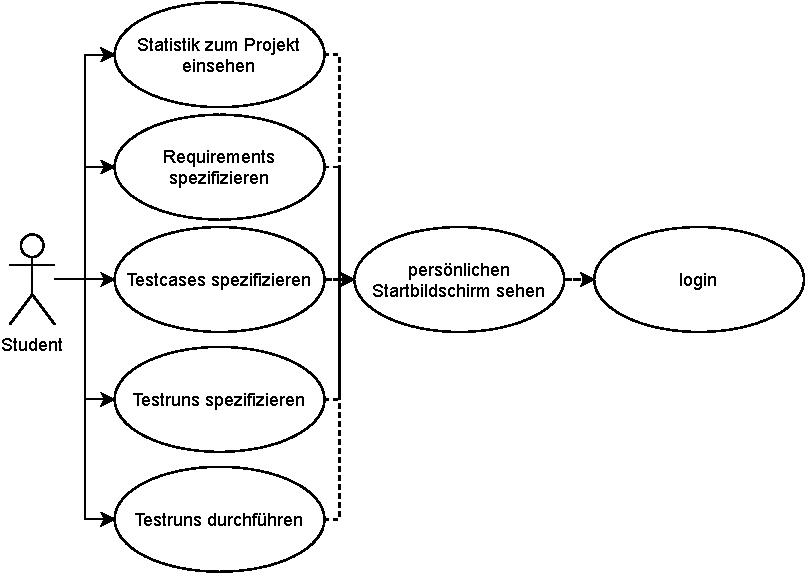
\includegraphics[width=1\textwidth]{usecase.pdf}
  \caption{Die Use cases des Studenten, eigene Darstellung}
  \label{f:usecase1}
\end{figure}


\begin{figure}[htpb]
  \centering
  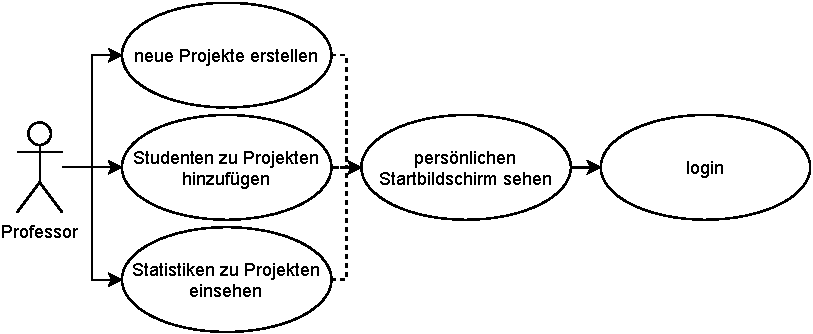
\includegraphics[width=1\textwidth]{usecase2.pdf}
  \caption{Die Use cases des Professors, eigene Darstellung}
  \label{f:usecase2}
\end{figure}

Basierend auf den Anforderungen wurden sowohl \textit{UML Use case Diagramme} als auch \textit{UML Aktivitätsdiagramme} erstellt. Zuerst wurden die \textit{Use cases} des Studenten in der Abbildung \ref{f:usecase1} gesammelt und die \textit{Use cases} des Professors in Abbildung \ref{f:usecase2} zusammengetragen. Alle \textit{Use cases} inkludieren dabei den \textit{Use case} "`persönlichen Startbildschirm einsehen"', welcher wiederum den \textit{Use case} "`login"' inkludiert.

\begin{figure}[htpb]
  \centering
  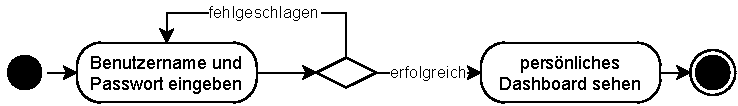
\includegraphics[width=1\textwidth]{activity.pdf}
  \caption{Login und persönlicher Startbildschirm, eigene Darstellung}
  \label{f:login}
\end{figure}


\begin{figure}[htpb]
  \centering
  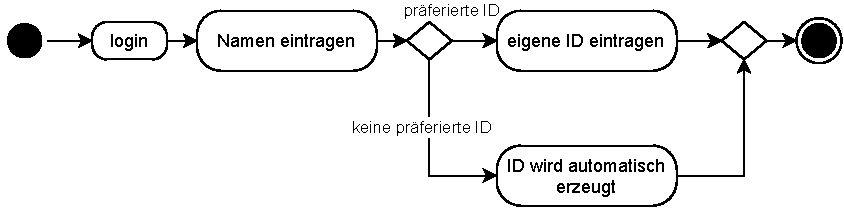
\includegraphics[width=1\textwidth]{activity2.pdf}
  \caption{neue Projekte erstellen, eigene Darstellung}
  \label{f:projekt}
\end{figure}

\begin{figure}[htpb]
  \centering
  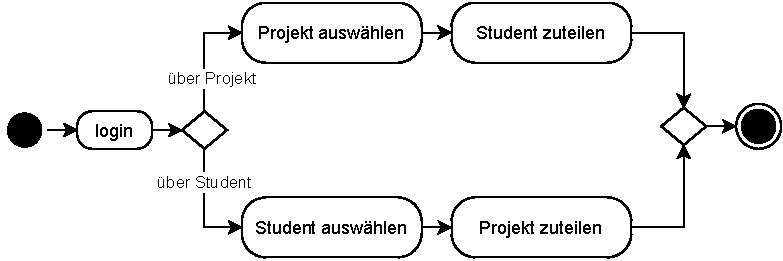
\includegraphics[width=1\textwidth]{activity3.pdf}
  \caption{Studenten zu Projekten hinzufügen, eigene Darstellung}
  \label{f:projektstud}
\end{figure}

\begin{figure}[htpb]
  \centering
  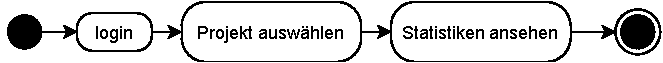
\includegraphics[width=1\textwidth]{activity4.pdf}
  \caption{Statistiken zu Projekten einsehen als Professor, eigene Darstellung}
  \label{f:projektstat}
\end{figure}

\begin{figure}[htpb]
  \centering
  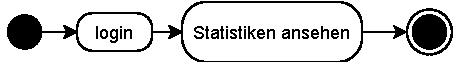
\includegraphics[width=1\textwidth]{activity45.pdf}
  \caption{Statistiken zu Projekten einsehen als Student, eigene Darstellung}
  \label{f:projektstatstud}
\end{figure}

\begin{figure}[htpb]
  \centering
  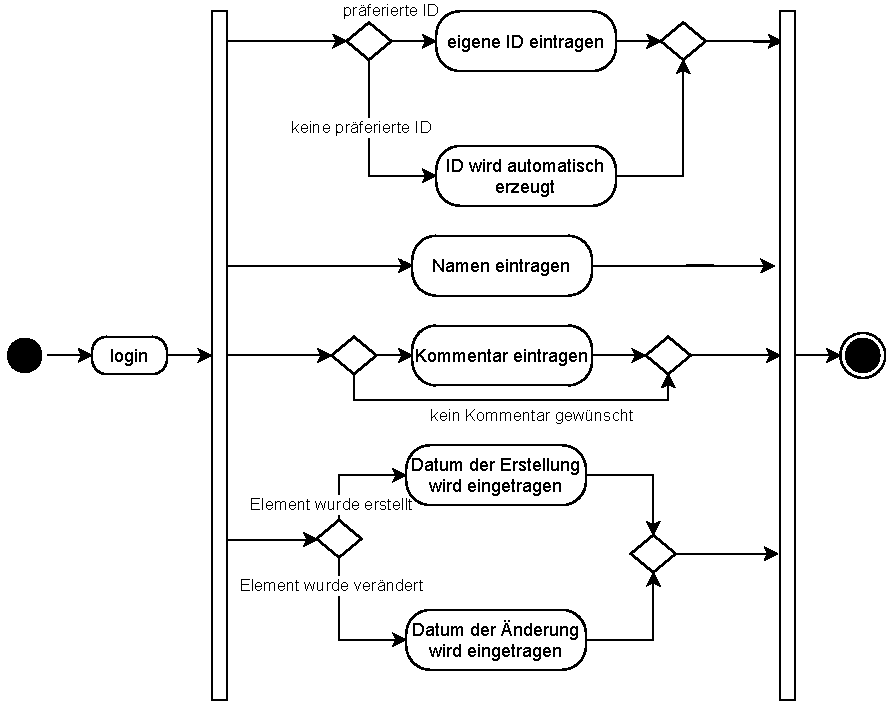
\includegraphics[width=1\textwidth]{activity6.pdf}
  \caption{Ein Element erstellen oder ändern, eigene Darstellung}
  \label{f:element}
\end{figure}

\begin{figure}[htpb]
  \centering
  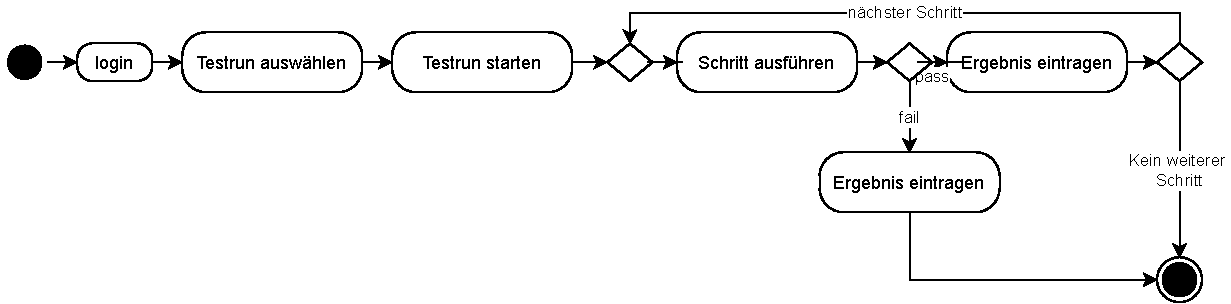
\includegraphics[width=1\textwidth]{activity7.pdf}
  \caption{Einen Testrun durchführen, eigene Darstellung}
  \label{f:testrun}
\end{figure}

Im nächsten Schritt wurden die \textit{Aktivitätsdiagramme} erstellt, welche verdeutlichen sollen, wie sich die Software zu verhalten hat. Angefangen beim Login aus der Abbildung \ref{f:login}, soll dieser solange nach einem Benutzername und Passwort fragen, bis das Einloggen schließlich erfolgreich ist. Die Anforderung A30, in der nach der Möglichkeit neue Projekte hinzuzufügen gefordert wird, ist in der Abbildung \ref{f:projekt} dargestellt. Hierbei kann ausgewählt werden, ob eine eigene, präferierte ID eingegeben werden soll. Die darauffolgende Anforderung A40, durch die es ermöglicht werden soll Studenten zu Projekten hinzuzufügen, ist in Abbildung \ref{f:projektstud} dargestellt. Es kann entweder das Projekt ausgewählt werden, um einen Studenten hinzuzufügen oder es kann ein Student ausgewählt werden, um ihn einem Projekt hinzuzufügen.

Die Statistiken sollen für Studenten bereits nach dem Login sichtbar sein, wie in Abbildung \ref{f:projektstatstud} zu sehen ist. Anders sieht es da beim Professor aus, dieser muss vorher noch eine Gruppe auswählen, um dann die Statistik zu sehen. Dieser Vorgang ist in der Abbildung \ref{f:projektstat} dargestellt.


Die Anfordeurngen aus dem Funktionsblock Anfoderungs- und Testmanagement wurden in der Abbildung \ref{f:element} zusammengetragen. Hier soll gezeigt werden, dass die verschiedenen Attribute eines Elements, wie zum Beispiel der Name oder gegebenenfalls ein Kommentar eingetragen werden können. Hierbei sind nur die Attribute dargestellt, die jedes Element besitzt. Besondere Attribute, wie die Kategorie des \textit{Requirement} wurden für diese Abbildung ausgelassen. Das letzte \textit{Aktivitätsdiagramm}, die Abbildung \ref{f:testrun}, zeigt den Ablauf bei der Durchführung eines \textit{Testruns}. Nach dem Login, dem Auswählen und Starten des \textit{Testruns} werden solange \textit{Testschritte} durchgeführt, bis es entweder keine \textit{Schritte} mehr gibt oder bis ein \textit{Schritt} nicht erfolgreich war. Wenn auch nur ein \textit{Schritt} nicht erfolgreich ist, so gilt der ganze \textit{Testrun} als durchgefallen.







\section{Entity-Relationship-Modell} \label{s:erm}

\begin{figure}[htpb]
  \centering
  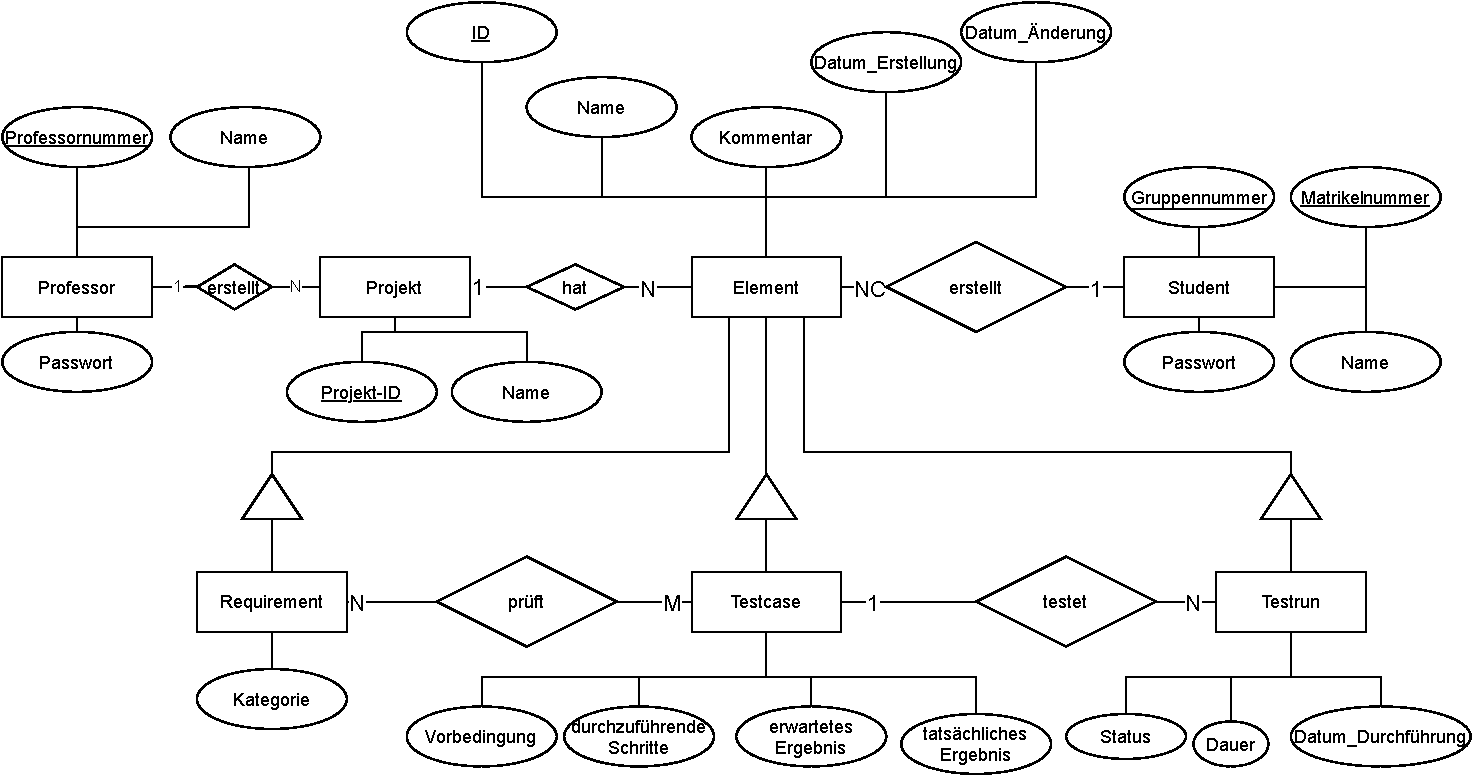
\includegraphics[width=1.2\textwidth]{er.pdf}
  \caption{Das Entity-Relationship-Modell, eigene Darstellung}
  \label{f:erd}
\end{figure}


In der Graphik \ref{f:erd} kann das \textit{Entity-Relationship-Modell} gesehen werden, das zur Grundlage des Datenbankdesigns dient. Im folgenden wird dieses Modell erklärt. Die \textit{Primary Keys} sind mit unterstrichenen Attributen dargestellt, während \textit{Foreign Keys} gestrichelte Unterstriche besitzen.


Damit sich ein Professor anmelden kann, braucht er eine Identifikation, wie eine Professorennummer, die ähnlich sein soll zu einer Matrikelnummer, sowie ein Passwort. Bei erfolgreicher Anmeldung wird sein Name angezeigt. Das Projekt wird von einem Professor erstellt, wobei ein Professor mehrere Projekte erstellen kann. Projekte haben eine ID und einen Namen, zum Beispiel "`Packstation"'. 

Ein Projekt kann mehrere Elemente haben, aber ein Element kann immer nur zu einem Projekt gehören. Die Elemente haben eine ID, einen Namen, einen Kommentar, ein Datum der Erstellung und ein Datum der letzten Änderung. Ein \textit{Requirement} ist ein Element und kann einer Kategorie zugeordnet werden. Ein \textit{Testcase} besitzt weitergehend die notwendigen Vorbedingungen für die durchzuführenden Schritte, das erwartete Ergebnis und das tatsächliche Ergebnis. Mehrere \textit{Testcases} können mehrere \textit{Requirements} abdecken. Ein \textit{Testrun} hat einen Status, der aussagt, ob der \textit{Testrun} erfolgreich ist oder nicht. Das ist realisierbar durch eine Auswahl zwischen den Möglichkeiten "`pass"' und "`fail"'. Daneben gibt ein \textit{Testrun} die Dauer an, die für ihn gebraucht wurde und das Datum an dem er durchgeführt wurde. Ein \textit{Testrun} testet immer nur einen \textit{Testcase}, aber ein \textit{Testcase} kann von mehreren \textit{Testruns} getestet werden. Ein Beispiel dazu ist, wenn der erste \textit{Testrun} nicht erfolgreich war und ein zweiter Versuch nötig ist. Der \textit{Testruns} kann nach der Durchführung nicht mehr geändert werden.

Ein Student braucht zur Anmeldung eine Matrikelnummer und ein Passwort, bei erfolgreicher Anmeldung wird sein Name angezeigt. Durch die Gruppennummer können Studenten in Gruppen auf die Projekte aufgeteilt werden. Die Gruppennummer soll dabei ein \textit{Foreign Key} auf die Projekt-ID sein. Ein Student kann ein, kein oder mehrere Elemente erstellen, aber ein Element wird immer nur einem Student zugeordnet.










\section{User-Interface-Prototyp} 
\label{s:ui}

\begin{figure}[htpb]
  \centering
  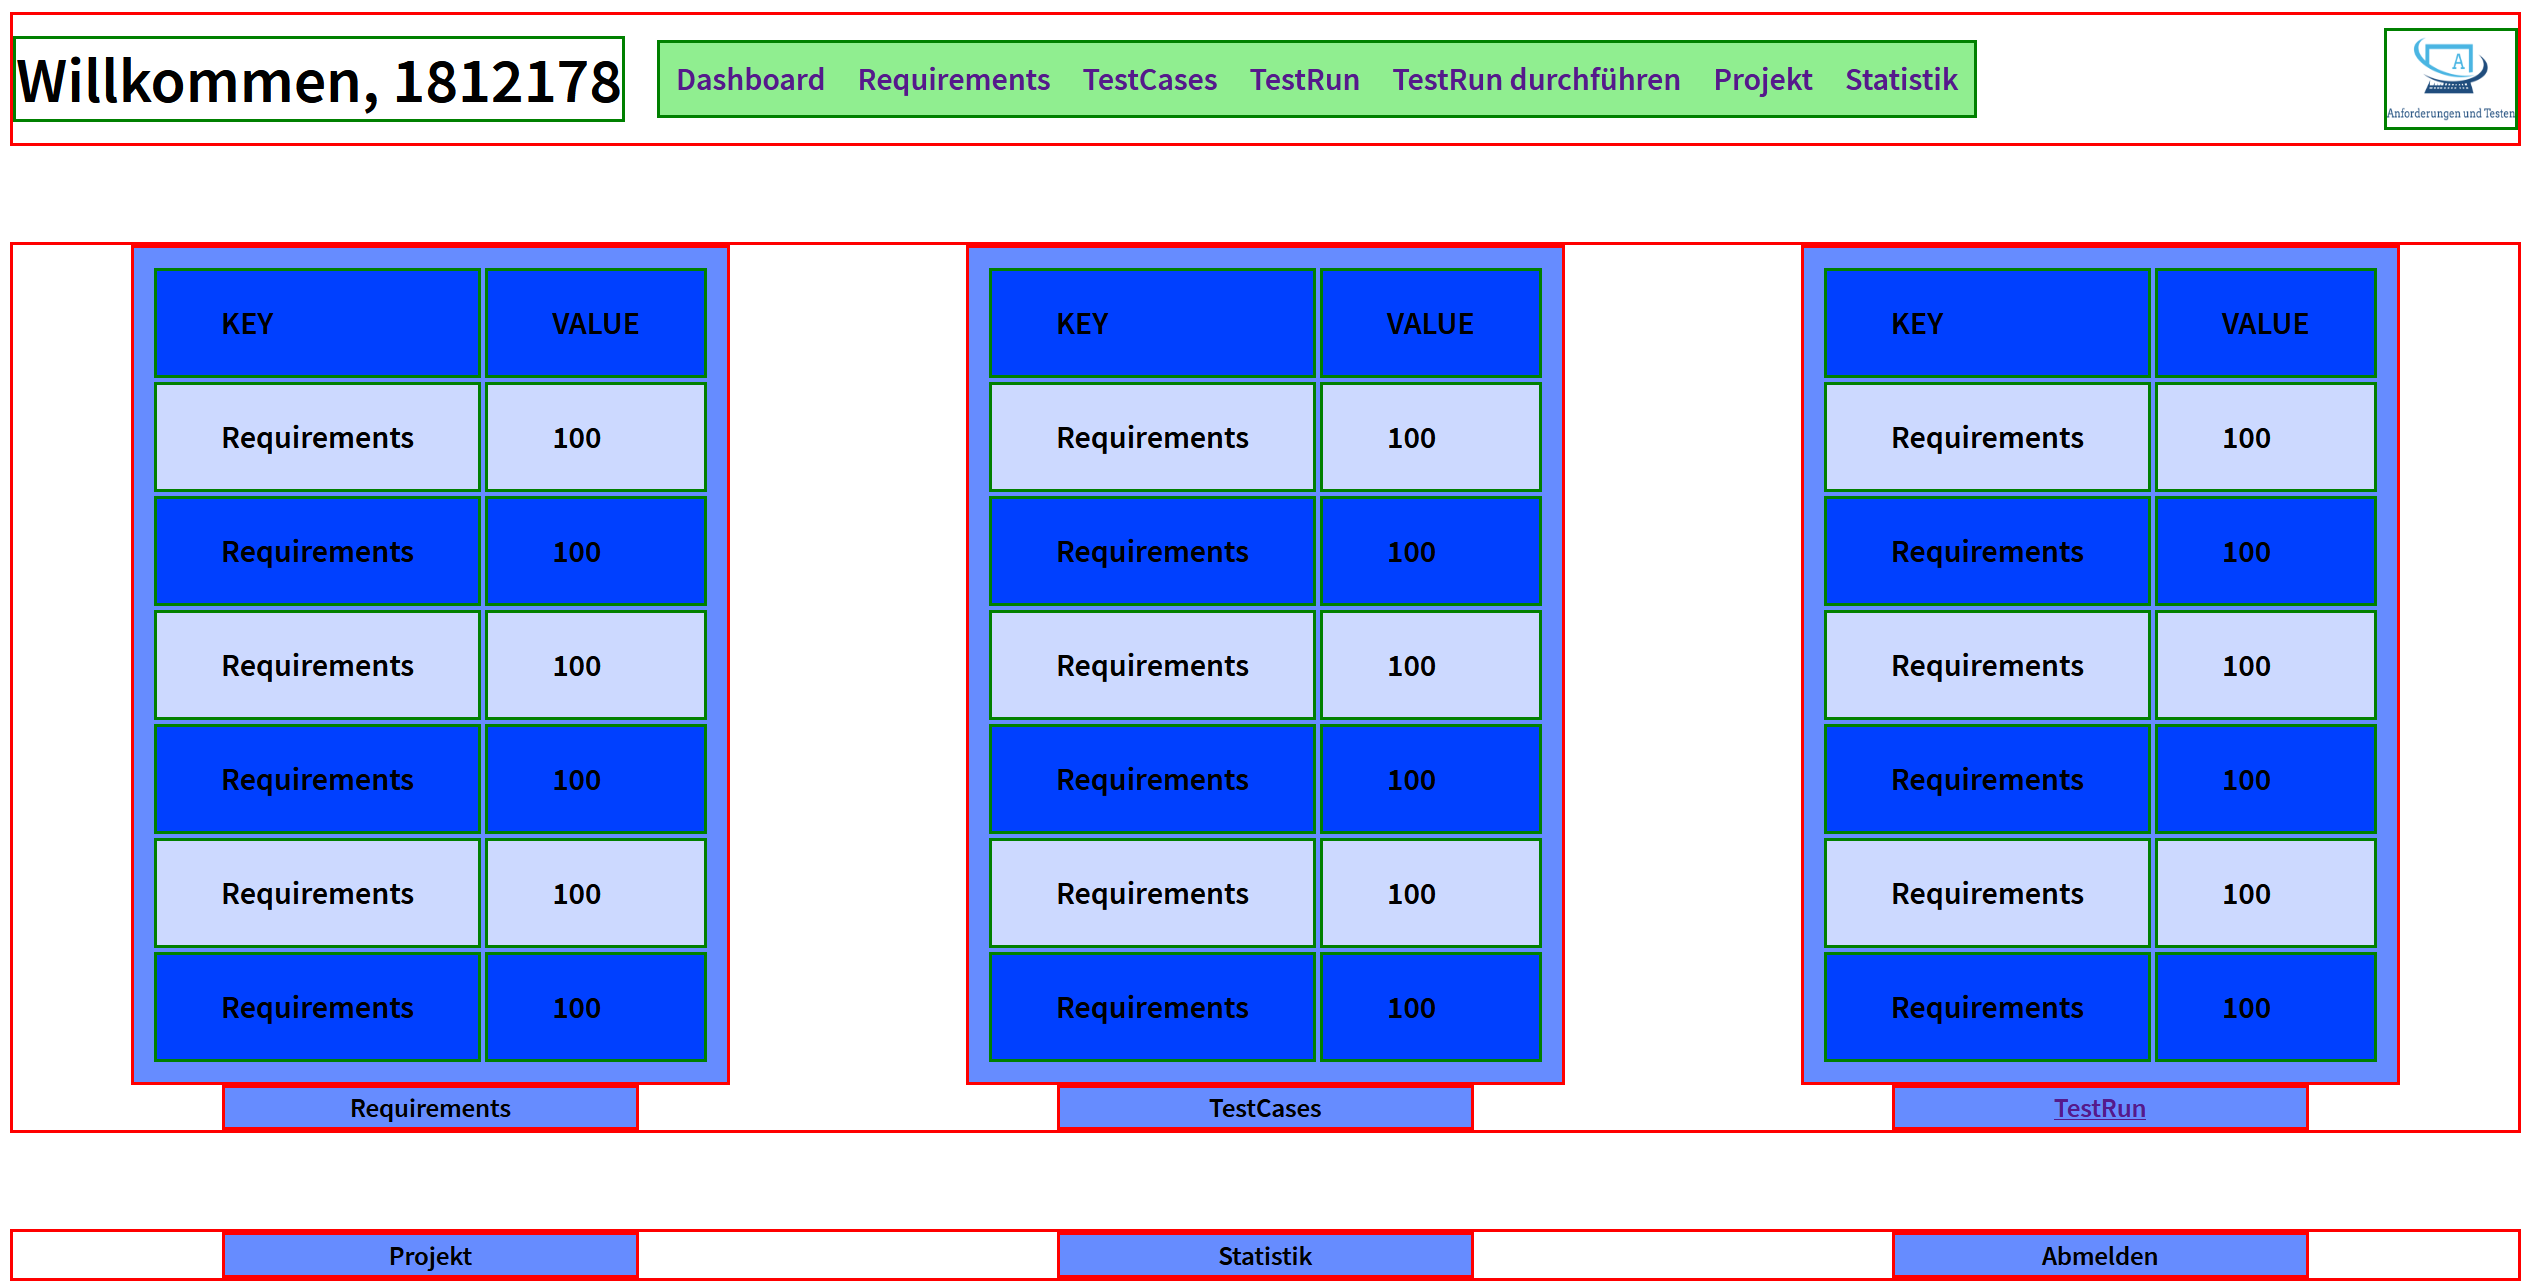
\includegraphics[width=1\textwidth]{pdash.png}
  \caption{Das Dashboard, eigene Darstellung}
  \label{f:pdash}
\end{figure}


\begin{figure}[htpb]
  \centering
  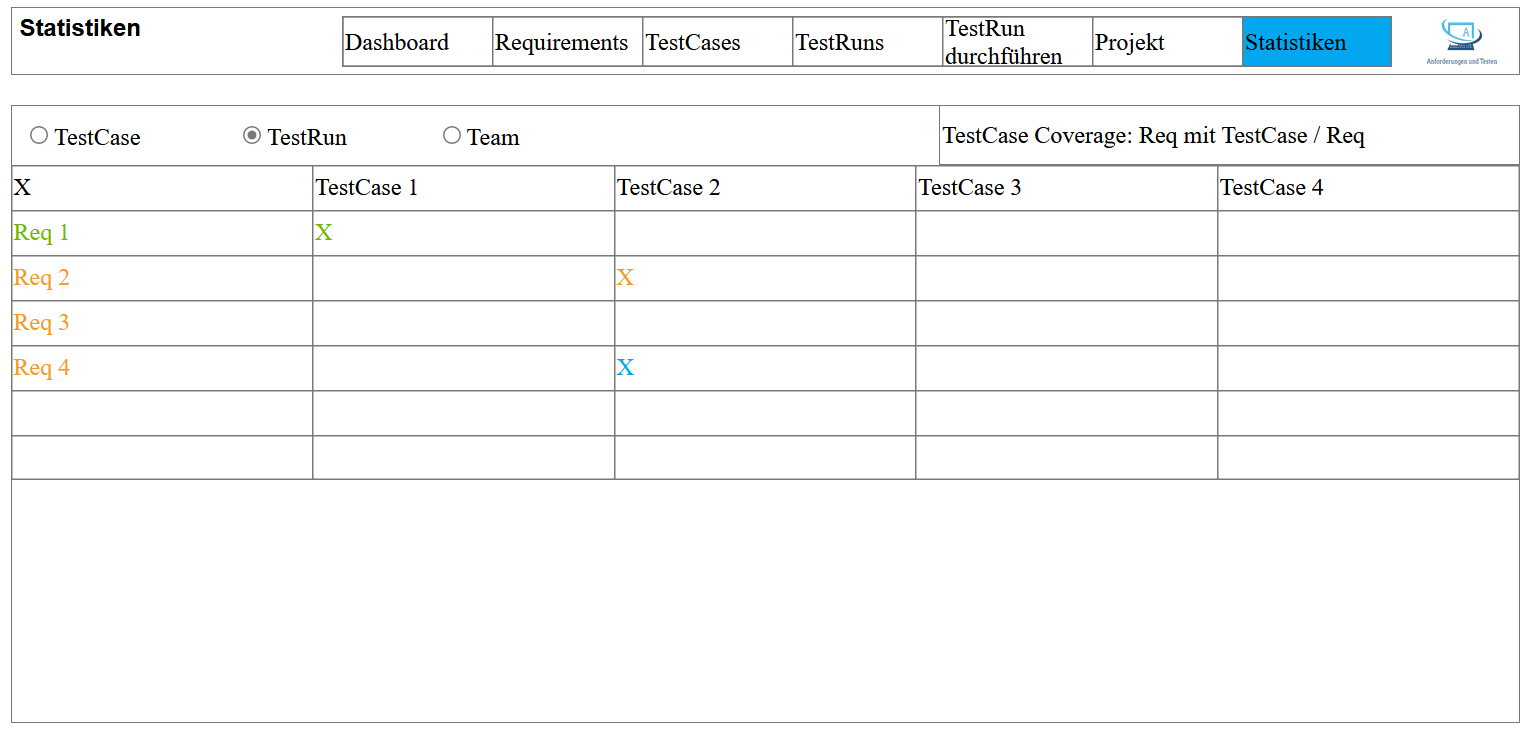
\includegraphics[width=1\textwidth]{pstat.png}
  \caption{Die Statistik Seite, eigene Darstellung}
  \label{f:pstat}
\end{figure}



\begin{figure}[htpb]
  \centering
  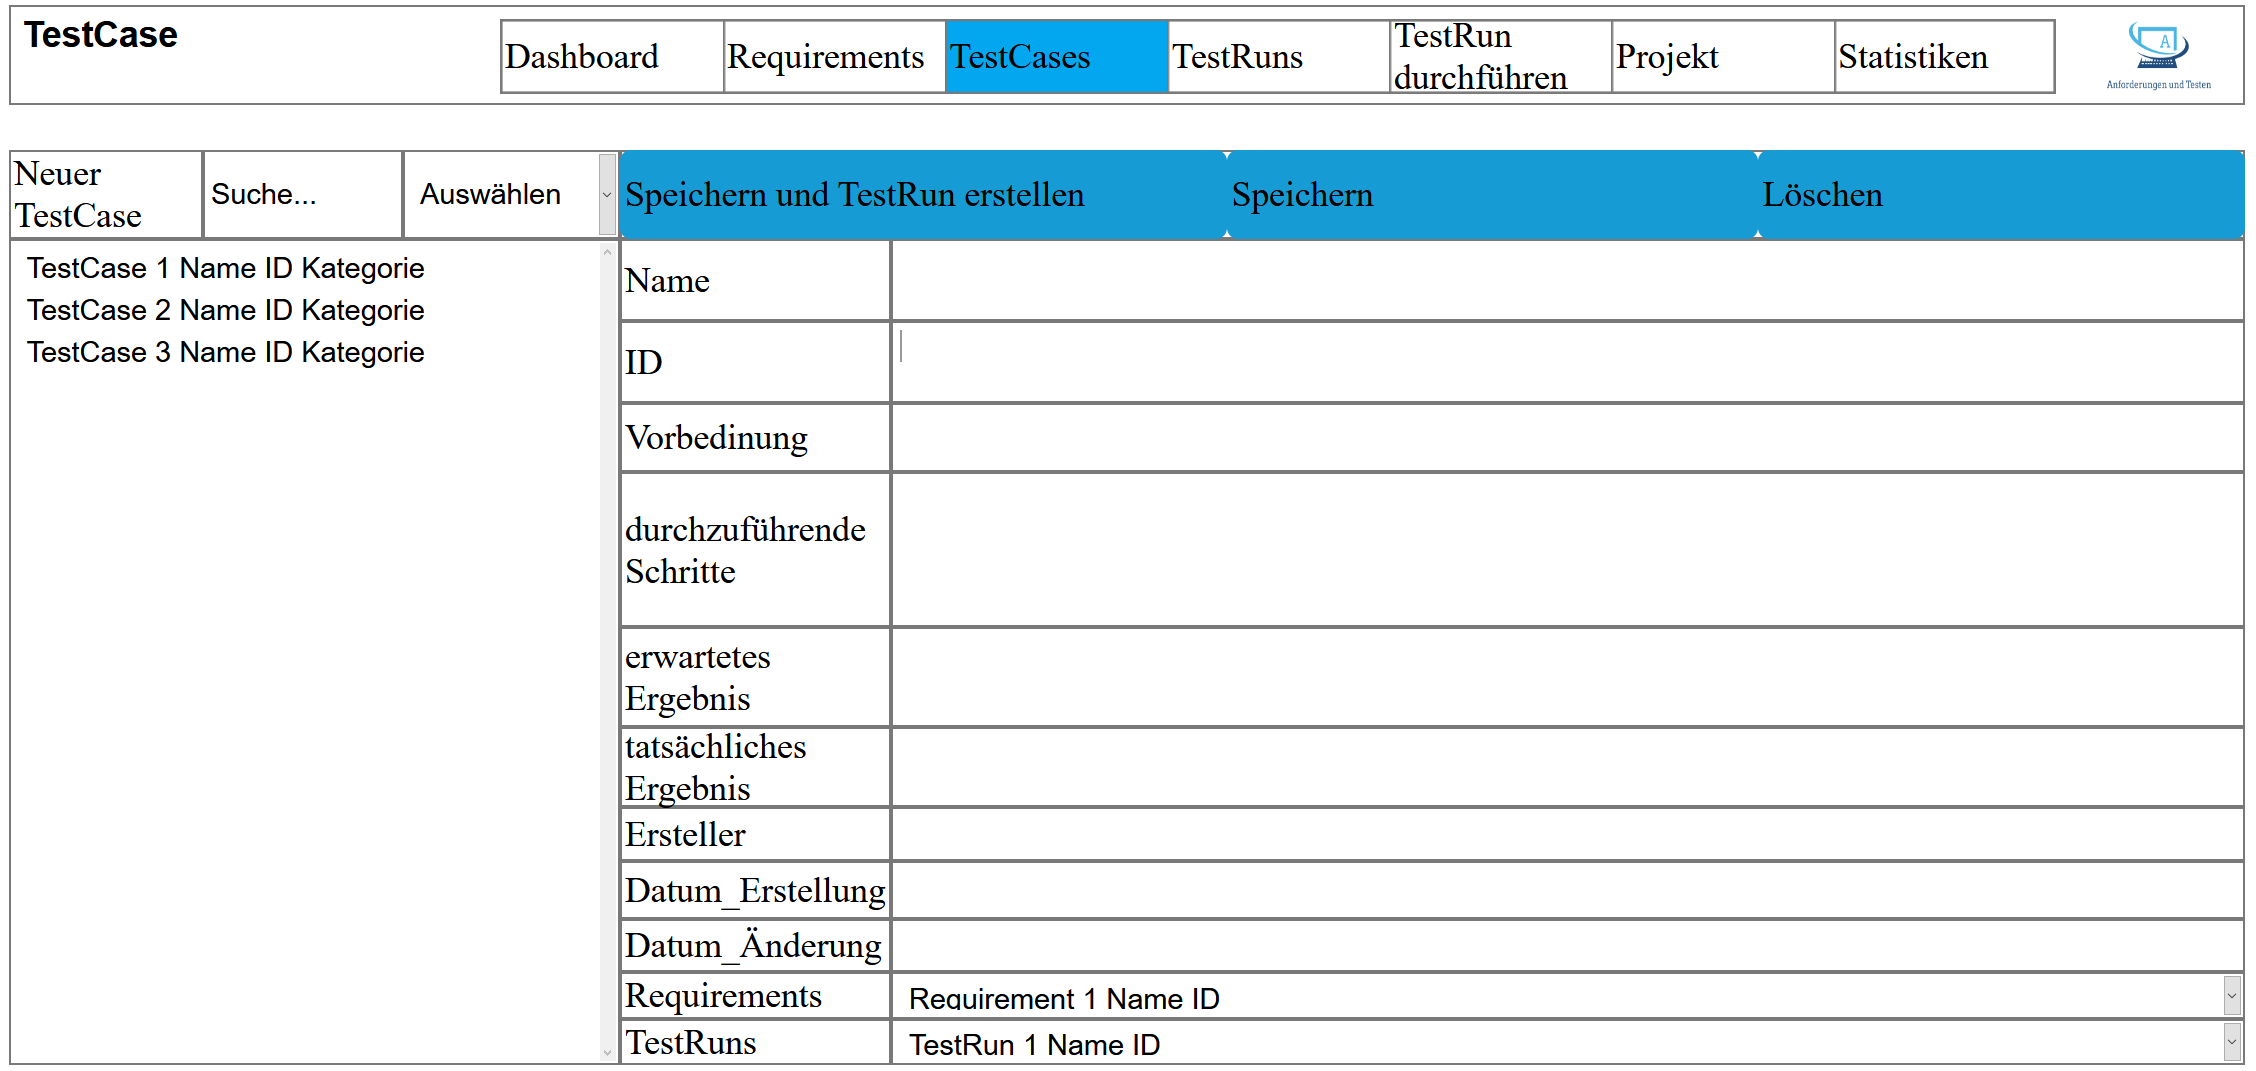
\includegraphics[width=1\textwidth]{ptestc.png}
  \caption{Die Erstellung eines Testcases, eigene Darstellung}
  \label{f:ptestc}
\end{figure}


\begin{figure}[htpb]
  \centering
  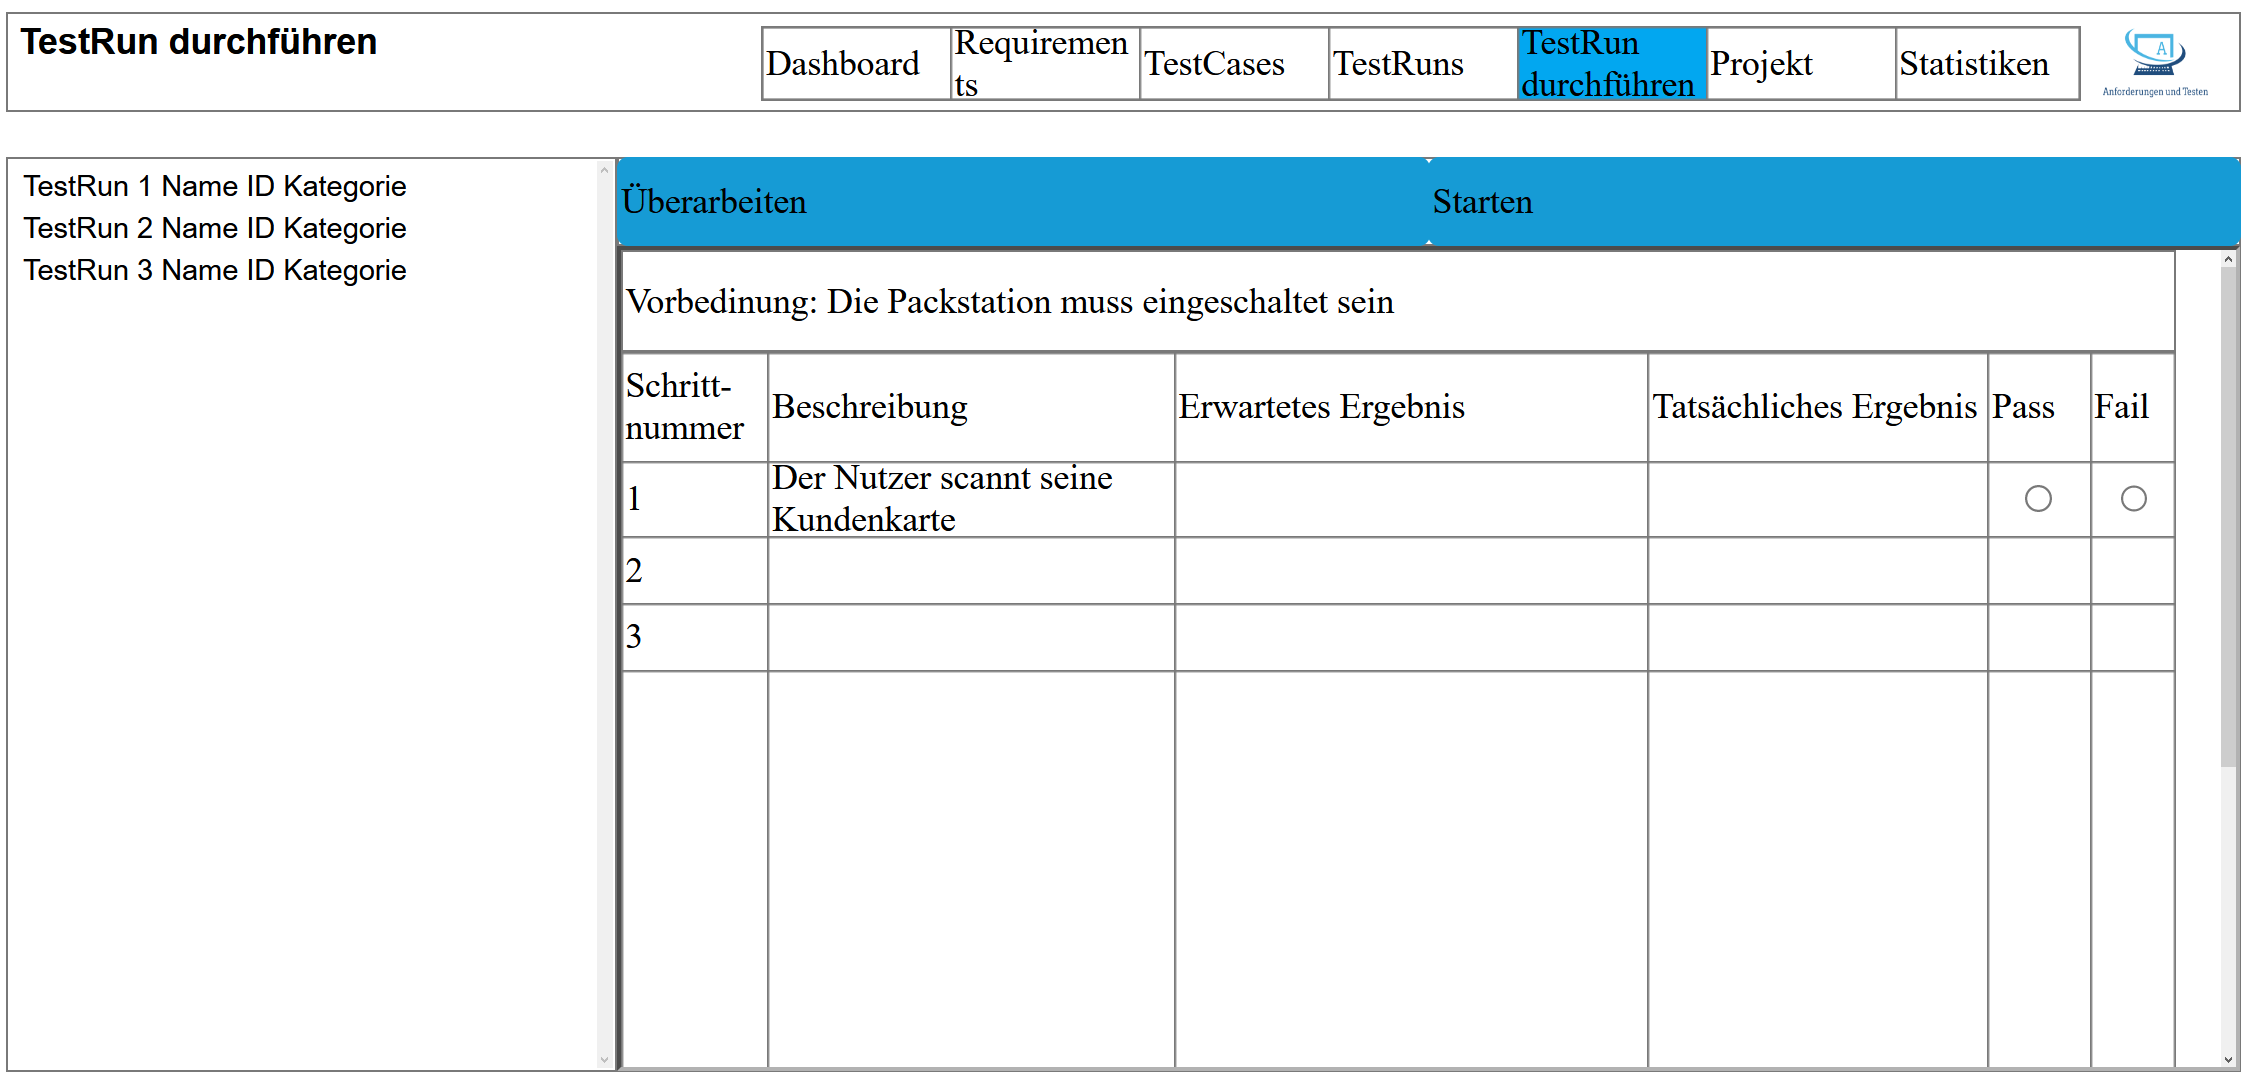
\includegraphics[width=1\textwidth]{ptestr.png}
  \caption{Die Durchführung eines Testruns, eigene Darstellung}
  \label{f:ptestr}
\end{figure}


Der Prototyp, um das \textit{User Interface} zu testen, wurde mit der kostenlosen Testversion der Software \textit{Axure RP 9} erstellt \cite{axure}. Mit dem entwickelten Prototypen konnte durch eine Demo ein erster Test zur \textit{Usability} gemacht werden. Der Prototyp basiert auf UI Skizzen, die auf der einen Seite selbst erstellt wurden und auf den UI Skizzen, die Herr Prof. Dr. Hastenteufel für das Projekt erstellt hat.

Auf den Abbildungen des Prototyps können bereits die grundlegenden Ideen zum Aufbau der Seite gesehen werden. Es soll eine Menüleiste am oberen Bildschirmrand geben, dabei soll die aktuelle Seite markiert sein. Für die \textit{Requirements}, \textit{Testcases} und die \textit{Testruns} soll es auf dem \textit{Dashboard} je eine Tabelle geben, wie in Abbildung \ref{f:pdash} gezeigt. Die angezeigten Daten sollen der Anforderung A40 entsprechen, beispielsweise wird die Anzahl der Anforderung pro Projekt visualisiert.

In der Anforderung A40 wurde auch eine Darstellung der verknüpften Elemente gefordert, also die \textit{Testfallabdeckung} und die \textit{Testabdeckung} der \textit{Requirements}. Nach den UI-Skizzen, die von Herrn Prof. Dr. Hastenteufel angefertigt wurden, sollte diese Anforderung durch eine \textit{Traceability-Matrix} realisiert werden.

Eine \textit{Traceability-Matrix} bietet die Möglichkeit die Verknüpfung zwischen den \textit{Requirements} und den \textit{Testcases} zu verfolgen. Sie wird darüber hinaus noch ergänzt durch die Information, welchen Status der \textit{Testrun} aufweist \cite{guru}.

In der Abbildung \ref{f:pstat} kann die \textit{Traceability-Matrix} gesehen werden. Sie ist aufgeteilt in zwei Ansichten. Die erste Ansicht zeigt nur die \textit{Requirements} und die \textit{Testcases}. Falls diese zusammengehören, gibt es in dem entsprechenden Feld ein X als Markierung dafür. In der zweiten Ansicht wird das X, das die Verknüpfung anzeigt mit den entsprechenden Farben markiert. Rot markierte Verknüpfungen zeigen an, dass der letzte \textit{Testrun} nicht erfolgreich war. Eine grüne Markierung signalisiert, dass der letzte \textit{Testrun} erfolgreich war. Daneben gibt es noch eine blaue Markierung, falls zu dem \textit{Testcase} noch keine \textit{Testruns} durchgeführt wurden.




In der nächsten Graphik \ref{f:ptestc} kann die Bearbeitung eines Elements gesehen werden, hier wird beispielsweise die Bearbeitung eines \textit{Testcases} gezeigt. Die Bearbeitungsseite für die \textit{Requirements}, \textit{Testcases} und \textit{Testruns} sollte für alle Elemente gleich aussehen. Es gibt aber pro Seite andere Attribute zum Eintragen, zum Beispiel kann beim \textit{Testcase} eine Vorbedingung eingetragen werden.


Zuletzt sei hier noch die Durchführung eines \textit{Testruns} in der Abbildung\ref{f:ptestr} gezeigt. Nachdem ein \textit{Testrun} aus der Liste an der linken Seite ausgewählt wurde, kann dieser ausgeführt werden. Dabei sind die Schritte in einer Tabelle angeordnet und zu jedem Schritt kann das tatsächliche Ergebnis und der Status eingetragen werden. Nur wenn alle Schritte erfolgreich durchgeführt werden konnten, wird der \textit{Testrun} insgesamt als erfolgreich angesehen. Wenn auch nur ein Schritt durchgefallen ist, dann ist auch der komplette \textit{Testrun} durchgefallen.


Es gab bei der Software \textit{Axure RP 9} die Option aus dem erstellten Prototypen die entsprechenden \textit{HTML-Seiten} zu generieren. Die auf diesem Weg generierten Seiten bestanden aber zu großen Teilen aus durchnummerierten \textit{div-Elementen}. Um eigene Anpassungen, beispielsweise durch \textit{CSS} zu machen, waren diese Seiten leider nicht brauchbar. Ein Beispiel dazu ist in dem Listing \ref{code:badhtml} dargestellt. In Zeile 26 kann das Wort "`Statistiken"' gesehen werden, das in der Statistik Seite oben links neben der Menüleiste angezeigt wird.


\begin{listing}[htbp]
\begin{lstlisting}
  <body>
    <div id="base" class="">

      <!-- Unnamed (Rectangle) -->
      <div id="u256" class="ax_default box_1">
        <div id="u256_div" class=""></div>
        <div id="u256_text" class="text " 
        style="display:none; visibility: hidden">
          <p></p>
        </div>
      </div>

      <!-- Unnamed (Rectangle) -->
      <div id="u257" class="ax_default box_1">
        <div id="u257_div" class=""></div>
        <div id="u257_text" class="text " 
        style="display:none; visibility: hidden">
          <p></p>
        </div>
      </div>

      <!-- Unnamed (Rectangle) -->
      <div id="u258" class="ax_default heading_1">
        <div id="u258_div" class=""></div>
        <div id="u258_text" class="text ">
          <p><span>Statistiken</span></p>
        </div>
      </div>
\end{lstlisting}
\caption{generierter HTML-Code der Statistik-Seite}
\label{code:badhtml}
\end{listing}






\chapter{Implementierung} 
\label{c:imp}

\textit{Django} wurde von einem Team, dass sich mit der Verwaltung von Zeitungsartikeln auf einer Webseite beschäftigt, dazu entwickelt, häufig auftretende Webentwicklungsaufgaben schnell und einfach realisieren zu können.  Auf die Idee kam das Team, als sich bei einer Vielzahl an Webseiten ein gleiches Design mit gleich aufgebautem Code sichtbar machte \cite{mozillatuto1}. Als \textit{Web-Framework} unterstützt \textit{Django} die Entwicklung von Webseiten, indem Dienste, wie die Datenbankanbindung, zur Verfügung gestellt werden \cite{webframe}. Ausgewählte Aspekte der Softwareentwicklung mit \textit{Django} sowie Ausschnitte des Codes sind an dieser Stelle erklärt.


\section{Einrichtung}

\begin{table}
\centering
\begin{tabular}{|p{0.3\textwidth}|p{0.7\textwidth}|}
\hline
\multicolumn{1}{|c|}{\textbf{Element}} & 
\multicolumn{1}{|c|}{\textbf{Version}} \\\hline
integrierte Entwicklungsumgebung/IDE & PyCharm Community 2020.2 \\\hline
Datenbank & PostgreSQL mit pgadmin 4.20 \\\hline
Programmiersprache & Python 3.7 \\\hline   
Web-Framework & Django 3.1.2 \\\hline   
\end{tabular}
\caption{Die benutzten Materialien für die Entwicklung der Software}
\label{t:tools}
\end{table}

In der Tabelle \ref{t:tools} sind die Materialien aufgelistet, die zur Erstellung des Tools verwendet wurden. Da \textit{Django} in \textit{Python} geschrieben ist, ist diese Programmiersprache die Grundvoraussetzung zum Arbeiten mit dem \textit{Web-Framework} \cite{djangotuto2}.


Zuerst muss in \textit{PyCharm} ein neues Projekt angelegt werden. Der Vorteil bei der Nutzung von \textit{PyCharm} als Entwicklungsumgebung ist, dass dabei auch direkt ein neues \textit{virtual environment} erstellt wird. Dadurch werden die Erweiterungen, die mit \textit{pip} installiert werden, nur für das aktuelle \textit{virtual environment} installiert und nicht global \cite{mozillatuto2}. Mit dem Befehl \verb|pip install django| kann \textit{Django} installiert werden \cite{djangotuto3}.


\begin{figure}[htpb]
  \centering
  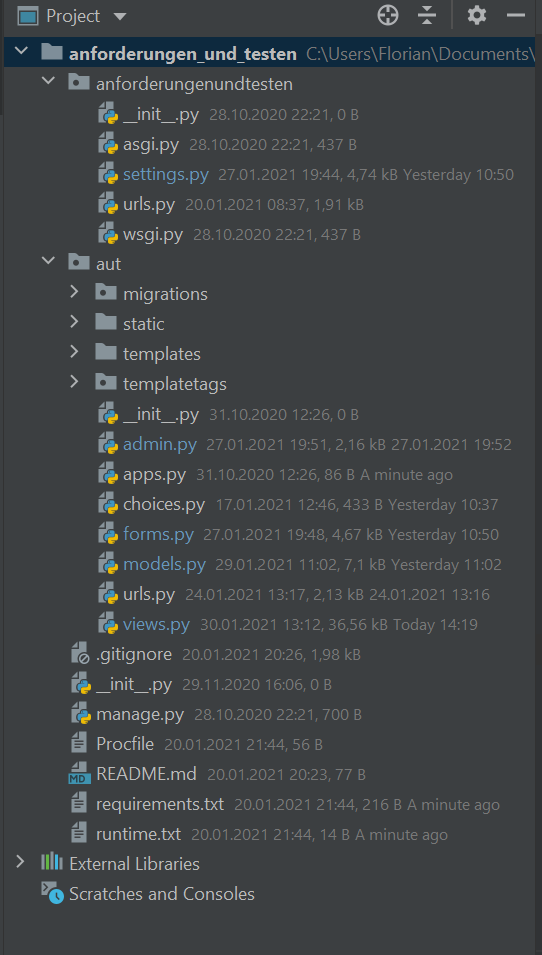
\includegraphics[width=1\textwidth]{files.png}
  \caption{Die komplette Struktur der Anwendung, eigene Darstellung}
  \label{f:files}
\end{figure}



\begin{table}
\centering
\begin{tabular}{|p{0.4\textwidth}|p{0.6\textwidth}|}
\hline
\multicolumn{1}{|c|}{\textbf{Datei/Ordner}} & 
\multicolumn{1}{|c|}{\textbf{Inhalt}} \\\hline
/anforderungen\_und\_testen & Der äußere Ordner ist ein Container für das Projekt, der Name ist nicht wichtig und kann beliebig umbenannt werden\\\hline
manage.py     & In dieser Datei sind die Kommandozeilenbefehle enthalten, wie zum Beispiel \verb|runserver| \\\hline
anforderungenundtesten/    & der innere Ordner ist das eigentliche Python Package \\\hline   

settings.py & Einstellungen die für das komplette Django Projekt gelten sind hier enthalten  \\\hline

urls.py & Die URLs für das gesamte Projekt sind in dieser Datei enthalten \\\hline
asgi.py & Für ASGI kompatible Webserver  \\\hline
wsgi.py & Für WSGI kompatible Webserver \\\hline

\end{tabular}
\caption{Die erstellten Inhalte nachdem ein neues Projekt erstellt wurde}
\label{tab:AutoCode}
\end{table}


Der Befehl ~\verb|django-admin startproject anforderungen_und_testen| erstellt ein neues \textit{Django-Projekt} und der dazu notwendige Code wird generiert. Dieser kann in der Tabelle \ref{tab:AutoCode} gesehen werden \cite{djangotuto3}. Ergänzend dazu ist in der Abbildung \ref{f:files} die komplette Projektstruktur abgebildet. 



\begin{figure}[htpb]
  \centering
  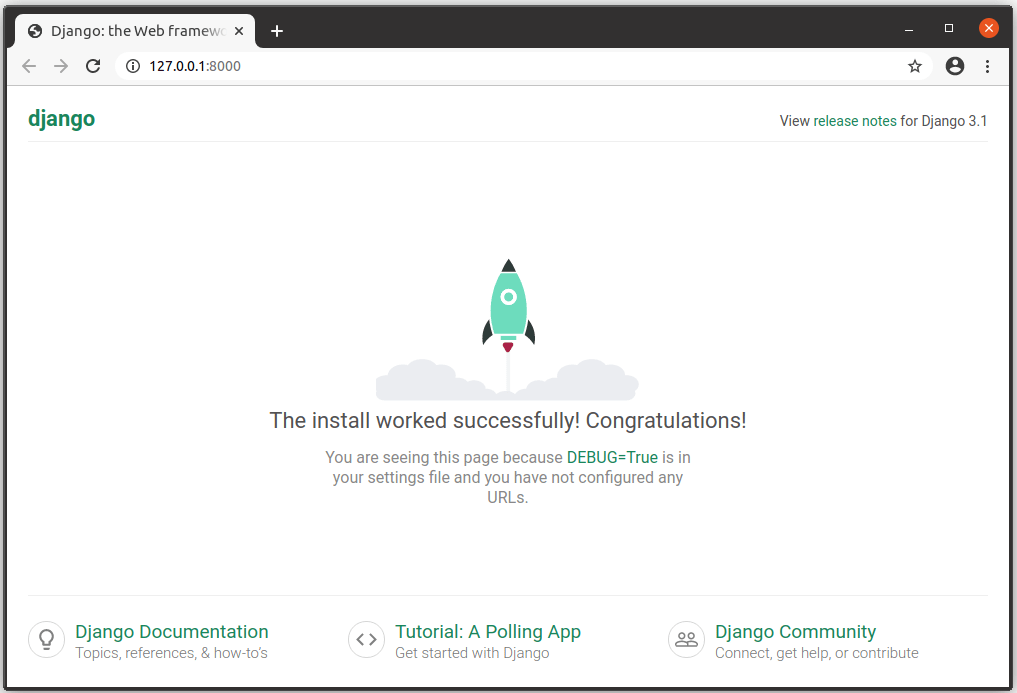
\includegraphics[width=1\textwidth]{rocket.png}
  \caption{Die Installation war erfolgreich, Abbildung aus \cite{mozillatuto2}}
  \label{f:rocket}
\end{figure}


Als nächstes wird der Befehl \verb|cd ./anforderungenundtesten| benutzt, um in den richtigen Ordner zu wechseln, welcher die \verb|manage.py| Datei enthält. Über den Befehl \verb|python manage.py runserver| kann der integrierte \textit{Development Server} von \textit{Django} gestartet werden. Falls die Abbildung \ref{f:rocket} zu sehen ist, ist die Installation erfolgreich \cite{djangotuto3}.


\begin{table}
\centering
\begin{tabular}{|p{0.3\textwidth}|p{0.7\textwidth}|}
\hline
\multicolumn{1}{|c|}{\textbf{Datei/Ordner}} & 
\multicolumn{1}{|c|}{\textbf{Inhalt}} \\\hline

/aut & Der Ordner beinhaltet die App\\\hline

\_\_init\_\_.py & Durch diese leere Datei wird der Ordner als Python Package registriert \\\hline

admin.py & In dieser Datei können die erstellten Modelle für den Admin registriert werden zum Bearbeiten\\\hline

apps.py & Die Datei enthält den Namen der App\\\hline

migrations/ & Der Ordner beinhaltet die Datenbankmigrationen\\\hline


models.py & Hier werden die Modelle definiert, die die Daten der Anwendung realisieren sollen\\\hline
views.py & die hier erstellten Funktionen werden über die URLs aufgerufen und befüllen die Templates mit Daten\\\hline
\end{tabular}
\caption{Die erstellten Dateien und Ordner nachdem eine App erstellt wurde}
\label{tab:AutoCode2}
\end{table}


Über den Befehl \verb|python manage.py startapp aut| wird eine neue \textit{App} angelegt wodurch weitere Dateien generiert werden. Diese sind in der Tabelle \ref{tab:AutoCode2} dargestellt und erklärt \cite{djangotuto3}. Es gibt einen Unterschied zwischen einem Projekt und einer \textit{App} in \textit{Django}. Eine \textit{App} ist eine \textit{Webanwendung}, die etwas machen kann. Während ein Projekt eine Ansammlung von Einstellungen und \textit{Apps} ist. Ein Projekt kann mehrere \textit{Apps} enthalten und eine \textit{App} kann in verschiedenen Projekten enthalten sein \cite{djangotuto3}.


Neben den automatisch erstellen Dateien und Ordnern mussten noch weitere Elemente erstellt werden, zum Beispiel die \verb|urls.py| Datei in der \textit{App}. Dadurch kann das Projekt auf die \textit{URLs} der \textit{App} zugreifen. Im Ordner \verb|static| befinden sich die auf der Webseite verwendeten Bilder, während sich die \textit{HTML-Dateien} in dem Ordner \verb|templates| befinden. Die Datei \verb|choices.py| beinhaltet die für die in \verb|forms.py| definierten \textit{Forms} benötigten Auswahlentscheidungen für die Nutzer. Zuletzt ist in dem Ordner \verb|templatetags| eine Datei enthalten in der sich die selbst geschriebenen \textit{Filter} befinden, welche in Kapitel \ref{s:itemp} erklärt sind. Wichtige Einstellungen in der \verb|settings.py| Datei beinhalten das Registrieren der \textit{App}, die Auswahl der Datenbank und das Einstellen der Sprache sowie der Zeitzone \cite{mozillatuto4}.



\section{Admin-Seite}


\begin{figure}[htpb]
  \centering
  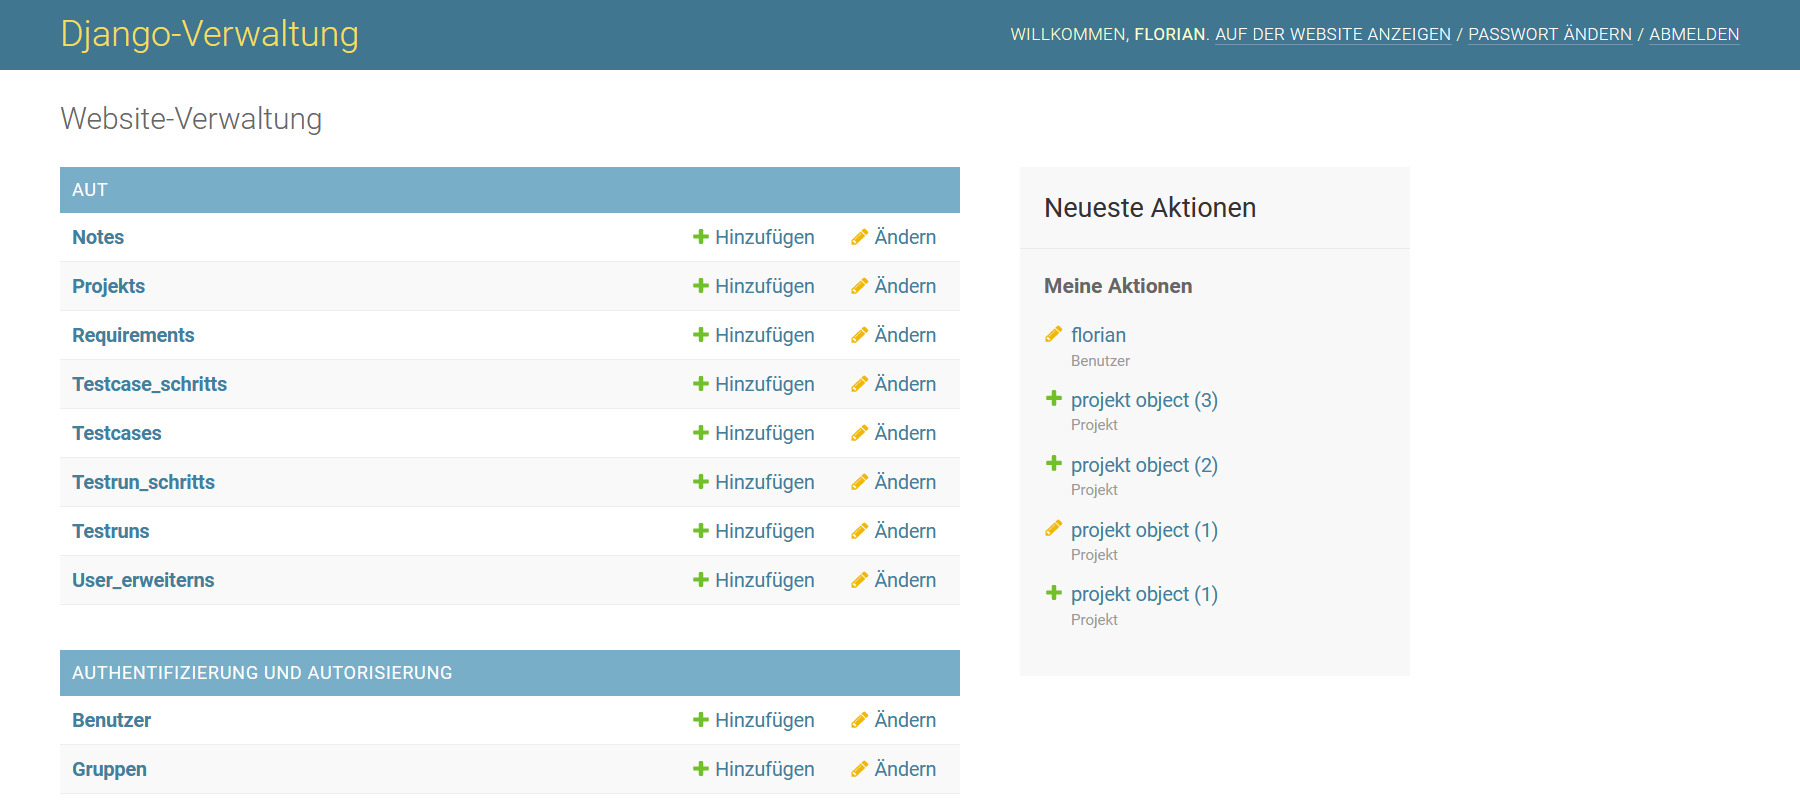
\includegraphics[width=1\textwidth]{admin.png}
  \caption{Die Admin-Seite, eigene Darstellung}
  \label{f:admin}
\end{figure}

Die Administrationsseite kann bei Bedarf automatisch von \textit{Django} erstellt werden. Mit dieser Seite können für die registrierten Modelle aus der \verb|admin.py| Datei Elemente hinzugefügt, gelöscht und geändert werden. Eine andere wichtige Funktion ist die Verwaltung der User der Webseite. Die Admin-Seite ist in der Abbildung \ref{f:admin} zu sehen. Für die Modelle können Berechtigungen hinzugefügt oder entfernt werden. Standardmäßig können alle angelegten Nutzer alle Modelle bearbeiten. Die Seite erfüllt den Zweck, dass kein eigenes \textit{Backend-Interface} erstellt werden muss, um Daten und Inhalte verwalten zu können. Außerdem ist es gedacht, diese Seite auch vom Kunden oder den Mitarbeitern im realen Umfeld benutzen zu lassen \cite{djangotuto4}. Der Befehl \verb|createsuperuser| erstellt einen Admin. Dazu muss noch ein Namen und ein Passwort eingegeben werden. Eine E-Mail ist optional einzugeben \cite{mozillatuto6}. Diese Seite wird auch in der Anwendung \textit{"`Anforderungen und Testen"'} verwendet, da so die Nutzerverwaltung bereits realisiert werden konnte. Die Anwendungsfälle für die Admin-Seite sind:
\begin{itemize}
\item Ein Nutzer hat sein Passwort vergessen und es muss wiederhergestellt werden.
\item Der Admin möchte eine neue Gruppe hinzufügen, wie in der Anforderung A20 gefordert.

\item Ein Nutzer möchte in eine andere Gruppe eingeteilt werden. Dieser Anwendungsfall basiert auf der Anforderung A30.

\end{itemize}





\section{URLs}
\label{s:iurl}

\begin{listing}[htbp]
\begin{lstlisting}
urlpatterns = [
    path('aut/', include('aut.urls')),
    path('', RedirectView.as_view(url='/aut/')),
]
\end{lstlisting}
\caption{URLs des Projekts}
\label{code:url1}
\end{listing}

Es gibt eine \verb|urls.py| Datei für das Projekt und eine pro \textit{App}. Von dem Projekt kann die Grundseite auf die Seite der App umgeleitet werden. Im Listing \ref{code:url1} wird zum einen die \verb|urls.py| Datei der \textit{App} inkludiert und zum Anderen der Hauptpfad des Projekts auf die \textit{App} umgelenkt. In dieser Arbeit ist der Hauptpfad "`aut"' \cite{mozillatuto5} .




\begin{listing}[htbp]
\begin{lstlisting}[
   basicstyle=\fontsize{8}{8}\selectfont\ttfamily
]
urlpatterns = [
    #Basis Views
    path('', views.view_dashboard, name='view_dashboard'),
    path('requirement', views.view_requirement, name='view_requirement'),
    path('testcase', views.view_testcase, name='view_testcase'),
    path('testrun', views.view_testrun, name='view_testrun'),
    path('statistik', views.view_statistik, name='view_statistik'),

    path('requirement/<int:pk>/', views.edit_requirement, name='requirement_change'),
    path('requirement/create/', views.edit_requirement, name='requirement_create'),
    path('requirement/create/<int:pk>/', views.edit_requirement, name='requirement_create'),
...
\end{lstlisting}
\caption{URLs der App}
\label{code:url2}
\end{listing}


In der \verb|urls.py| Datei der \textit{App}, von der ein Ausschnitt im Listing \ref{code:url2} zu sehen ist, wird jeweils eine \textit{URL} oder ein \textit{URL-Schema} mit einer Funktion aus der \verb|views.py| Datei verknüpft. Hierbei können noch Parameter angegeben werden, die an die \textit{View-Funktionen} übergeben werden sollen. Sobald eine URL übereinstimmt, wird die damit verknüpfte \textit{View} aufgerufen \cite{djangotuto1}.


\section{Modelle}



\begin{listing}[htbp]
\begin{lstlisting}[
   basicstyle=\fontsize{8}{8}\selectfont\ttfamily
]
class requirement(models.Model):
    #Private Keys, Foreign Keys and andere Beziehungen:
    req_pk_requirementid = models.AutoField(primary_key=True, null=False, unique=True)
    req_fk_ersteller = models.ForeignKey(User, on_delete=models.SET_NULL, null=True, blank=True)

    #Atrribute:
    req_name = models.CharField(max_length=100, null=True, blank=True)
    req_kommentar = models.CharField(max_length=300, null=True, blank=True)
    req_datum_erstellung = models.DateTimeField(auto_now_add=True, null=True, blank=True)
    req_datum_aenderung = models.DateTimeField(auto_now=True, null=True, blank=True)
    req_beschreibung = models.CharField(max_length=300, null=True, blank=True)

    #Funktionen:
    def __str__(self):
        return "r_" + str(self.req_pk_requirementid) + ": " + str(self.req_name)

    def get_id(self):
        return "r_" + str(self.req_pk_requirementid)

    def get_absolute_url(self):
        return reverse('aut:requirement_change', args=[str(self.req_pk_requirementid)])

    #Metaoptionen
    class Meta:
        ordering = ["req_pk_requirementid"]


\end{lstlisting}
\caption{URls der App}
\label{code:req}
\end{listing}

Die Modelle der \textit{App} werden basierend auf dem zuvor definierten \textit{ER-Modell} aus Kapitel \ref{s:erm} erstellt mit leichten Abwandlungen. Im Listing \ref{code:req} ist das Modell der \textit{Requirements} angegeben. An diesem Beispiel soll das Beschreiben der Modelle durch \textit{Django} erklärt werden. Der \textit{Primary-Key} wird normalerweise automatisch generiert, aber damit ein verständlicherer Name benutzt werden kann, wurde dieser überschrieben. Die \textit{Foreing-Keys} benötigen als besonderes Merkmal nur den Namen des anderen Modells das sie referenzieren. Die weiteren Attribute wurden mit den Standard Feldern, wie zum Beispiel \verb|Charfield|, definiert. Jedem Feld können außerdem Attribute zugewiesen werden. Die wichtigsten Attribute sind \verb|blank=True| und \verb|null=True|. Durch diese beiden Attribute dürfen die Felder sowohl leer sein, als auch in den \textit{Forms} leer angezeigt werden \cite{mozillatuto5}. Es kann gesehen werden, dass die "`is-a"'-Beziehung dadurch realisiert wurde, dass die \textit{Requirements}, \textit{Testcases} und \textit{Testruns} alle die allgemeinen Attribute der Relation Element aus dem \textit{ER-Diagramm} erhalten haben. Diese Realisierungsart war einfacher, da so keine \textit{JOIN-Operationen} ausgeführt werden müssen, wenn beispielsweise die allgemeinen Attribute wie der Name eines \textit{Testruns} gebraucht werden.


Neben den normalen Feldern, können in den Modellen auch noch Methoden und Metadaten definiert beziehungsweise angegeben werden. Eine generelle wichtige Funktion, die implementiert werden sollte, ist das Überschreiben der \verb|__str__| Funktion, da sie angibt, wodurch die Elemente repräsentiert werden sollen \cite{mozillatuto5}. Die andere Funktion \verb|get_absolute_url| kann dazu genutzt werden zu jedem \textit{Requirement} die entsprechende \textit{URL} anzugeben, die zu der Bearbeitungsseite führt und den \textit{Private-Key} als Parameter übergibt. Durch diese Beschreibung der Modelle kann \textit{Django} die entsprechenden Tabellen erstellen und übernimmt die Kommunikation mit der Datenbank \cite{djangotuto4}.


\begin{listing}[htbp]
\begin{lstlisting}[
   basicstyle=\fontsize{8}{8}\selectfont\ttfamily
]
class user_erweitern(models.Model):
    user = models.OneToOneField(User, on_delete=models.CASCADE, null=True, blank=True)
    gruppennummer = models.ForeignKey('projekt', on_delete=models.SET_NULL, null=True, blank=True)
    rolle = models.CharField(max_length=1, choices=ROLLEN, null=True, blank=True)
\end{lstlisting}
\caption{Die Erweiterungen des Users}
\label{code:user}
\end{listing}


Um den Nutzer zu implementieren wurde das vorgegebene \textit{User-Modell} von \textit{Django} erweitert. Die Erweiterungen sind in dem Listing \ref{code:user} zu sehen. Um die Elemente den einzelnen Gruppen zuzuordnen, brauchte der Nutzer das Attribute \verb|gruppennummer|. Das Attribut ist dabei ein \textit{Foreign-Key} auf die erstellten Projekte. Eine Abweichung vom \textit{ER-Modell} stellt die Realisierung der Studenten und des Professors dar. Da beide Nutzergruppen im \textit{ER-Modell} als eigene Relationen definiert sind, sollten sie in der Implementierung eigene Modelle erhalten. Stattdessen hat es sich angeboten das \textit{User-Modell} um das Attribut \verb|rolle| zu erweitern.



Nachdem die Modelle erstellt wurden, müssen die Befehle \verb|makemigrations| und \verb|migrate| angewandt werden, da so sämtliche Änderungen an den Modellen ausgeführt werden. Mit \verb|makemigrations| werden die \verb|migration|-Dateien erstellt, um gegebenenfalls die Befehle zu kontrollieren, die von \textit{Django} erstellt wurden. Das Ausführen der Migration geschieht durch den Befehl \verb|migrate|. Damit werden alle notwendigen Tabellen erstellt und Änderungen durchgeführt \cite{djangotuto4}.



\section{Views}
\label{iviews}

\begin{figure}[htpb]
  \centering
  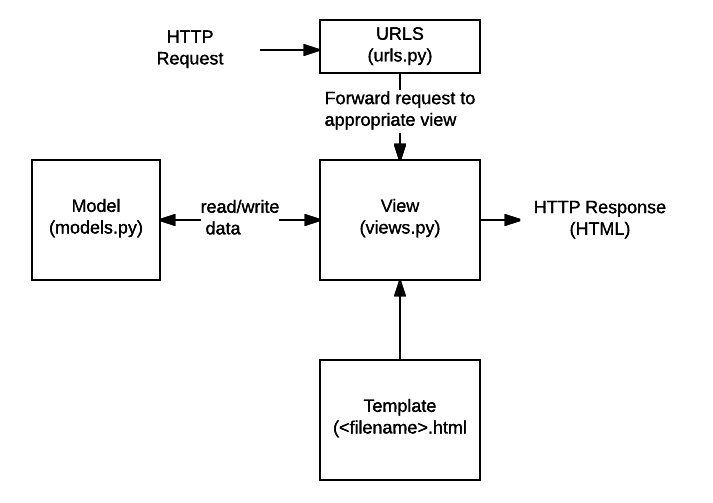
\includegraphics[width=1\textwidth]{django_basic.png}
  \caption{Der generelle Ablauf eines HTTP Requests, aus \cite{mozillatuto1}}
  \label{f:django_basic}
\end{figure}

Der generelle Ablauf bei einem \textit{HTTP Request} ist in der Darstellung \ref{f:django_basic} abgebildet. In \textit{Django Applikationen} werden die verschiedenen Aufgaben auf verschiedene Dateien aufgeteilt. Die \textit{URLs} werden mit den entsprechenden \textit{Views} verlinkt. Darüber hinaus können bestimmte Parameter aus der \textit{URL} an die \textit{Views} zum weiteren Verarbeiten übergeben werden. In den \textit{Views} können die benötigten Daten, die als Modelle in der \verb|models.py| Datei definiert sind, angegeben werden. Die \textit{HTML-Templates} werden dann im nächsten Schritt mit diesen Daten basierend auf der Logik in den \textit{Views} befüllt, dafür haben sie an den entsprechenden Stellen befüllbare Platzhalter. Abschließend generiert die \textit{View} die \textit{HTTP Response}. Diese Aufteilung wird "`Model View Template"' Architektur genannt \cite{mozillatuto1} und kann mit der "`Model View Controller"' Architektur verglichen werden \cite{mvc}.


\begin{listing}[htbp]
\begin{lstlisting}[
   basicstyle=\fontsize{7}{7}\selectfont\ttfamily
]
def view_requirement(request):
    users = User.objects.filter(user_erweitern__gruppennummer=request.user.user_erweitern.gruppennummer)
    req_for_usergroup = requirement.objects.filter(req_fk_ersteller__in=users).order_by('-req_pk_requirementid')

    context = {
        'requirements': req_for_usergroup,
    }
    return render(request, 'aut/010_requirement.html', context=context)
\end{lstlisting}
\caption{View-Funktion der Requirements Seite, eigenen Darstellung}
\label{code:allrequirements}
\end{listing}




\begin{figure}[htpb]
  \centering
  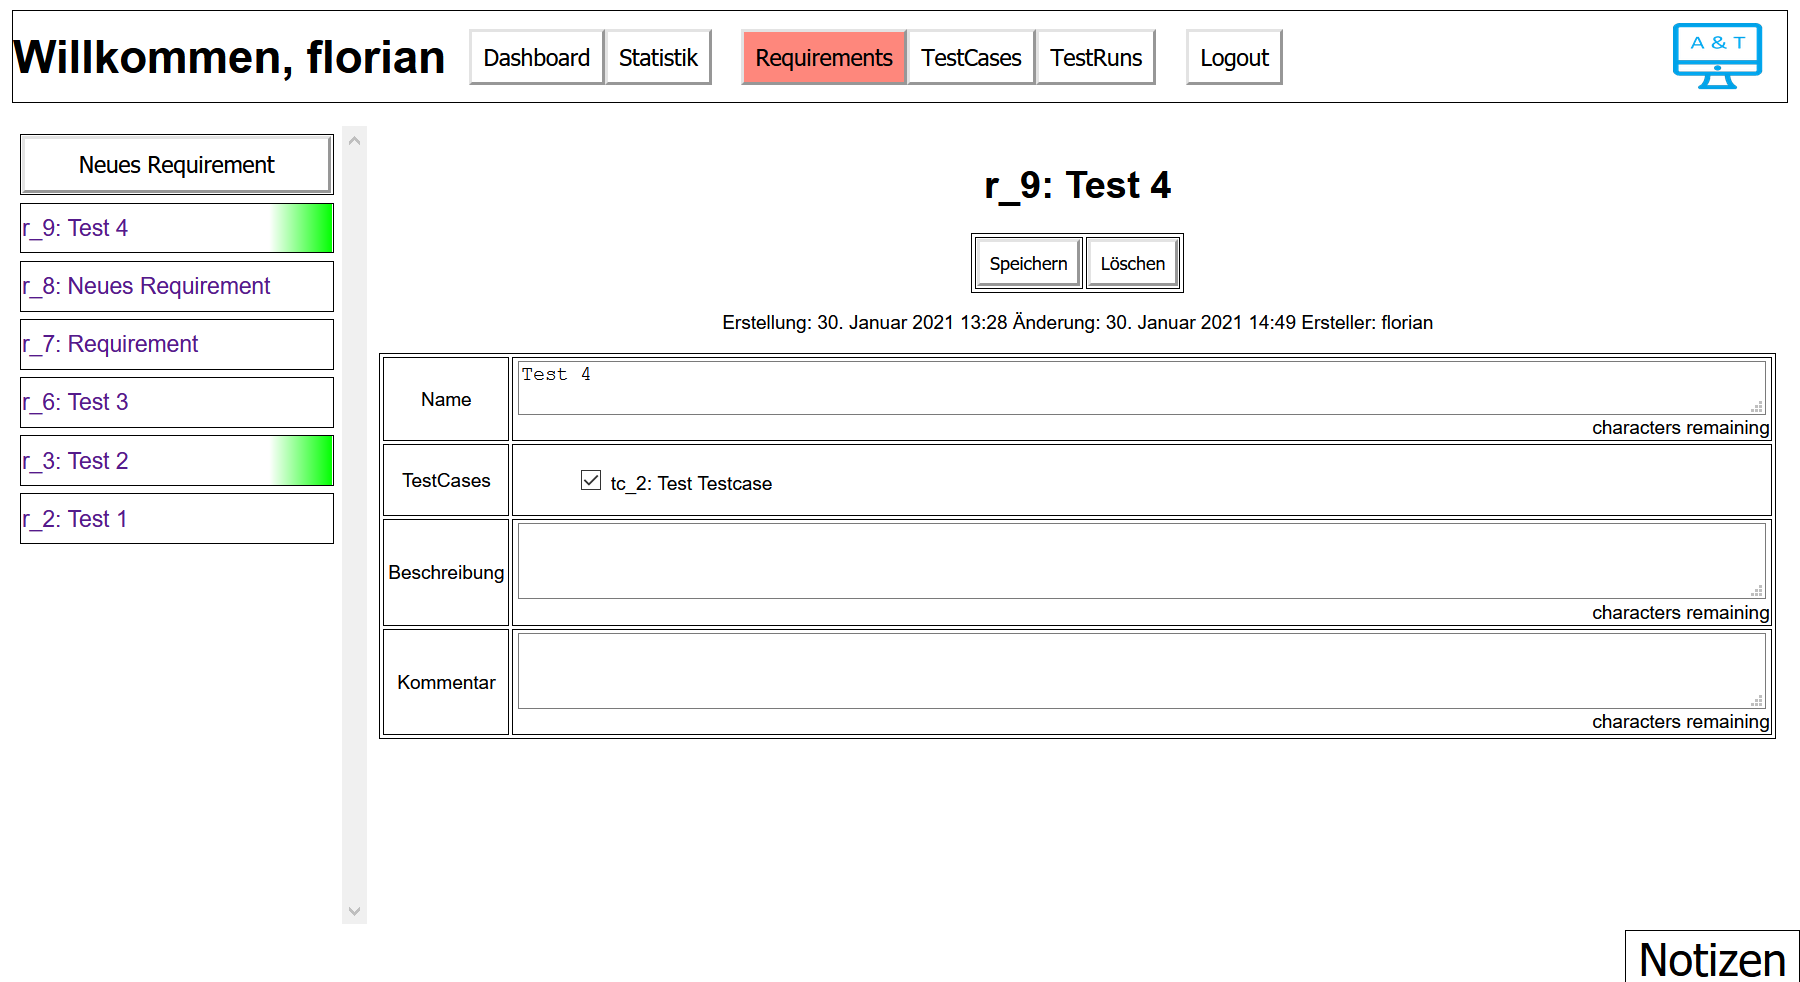
\includegraphics[width=1\textwidth]{softreqs.png}
  \caption{Requirements-Liste auf der Requirements Seite, eigene Darstellung}
  \label{f:softreqs}
\end{figure}



Beispielsweise ist in Listing \ref{code:allrequirements} die \textit{View} dargestellt, um alle \textit{Requirements} einer Usergruppe herauszufiltern. Die einzelnen \textit{Views} sind als Funktionen in \textit{Python} definiert \cite{mozillatuto1}. Zuerst werden in Zeile zwei alle Nutzer mit der gleichen Gruppennummer herausgefiltert, bevor die \textit{Requirements} aller Nutzer aus der Datenbank geholt werden. Die \textit{Requirements} werden dann noch in Zeile 3 nach absteigender Folge der IDs sortiert, damit die neuesten \textit{Requirements} in der Liste oben stehen. Wenn diese Variable an das \textit{Template} übergeben werden soll, dann muss sie im \textit{Context} angegeben werden. Es wird ein Name in Anführungsstrichen angegeben, der dann im \textit{Template} benutzt werden kann. Der Einfachheit halber wurde immer derselbe Name, wie der, der Variablen verwendet. Zusammen mit dem \textit{Template} muss dieser \textit{Context} dann zum rendern in der Zeile acht aufgerufen werden. In der Abbildung \ref{f:softreqs} kann die auf diesem Weg erstellt Liste am linken Bildschirmrand gesehen werden. Der nähere Aufbau der \textit{Templates} ist im Kapitel \ref{s:itemp} beschrieben.




\begin{listing}[htbp]
\begin{lstlisting}[
   basicstyle=\fontsize{7}{7}\selectfont\ttfamily
]
def edit_requirement(request, pk=None):
    requ_instance, created = requirement.objects.get_or_create(req_pk_requirementid=pk)
    if created == True:
        requ_instance.req_fk_ersteller = request.user
        requ_instance.save()
        ...
\end{lstlisting}
\caption{View-Funktion der Requirements Seite}
\label{code:editreq}
\end{listing}


Eine weitere \textit{View}, die eine andere Möglichkeit von \textit{Django} präsentiert, ist in dem Listing \ref{code:editreq} dargestellt. Hierbei wurde aus der \textit{URL} noch ein Parameter übergeben und kann in der Funktion als Variable benutzt werden. Gebraucht wurde diese Funktionalität, damit sowohl neu erstellte Elemente, die zum Beispiel durch den Button "`Neues Requirement"' aus der Abbildung \ref{f:softreqs} erstellt werden, als auch bereits vorhandene Elemente, bearbeitet werden können. Neu erstellte Elemente besitzen noch keinen \textit{Private-Key}, da sie noch nicht abgespeichert wurden. Dafür bekommen sie den default Wert \textit{None} aus Zeile eins als \textit{Private-Key}. Ein bereits vorhandenes Element würde an dieser Stelle seinen \textit{Private-Key} angeben, zum Beispiel kann das Element "`r\_2: Test 1"' über seinen \textit{Private-Key} zwei erhalten werden. Die Funktion \verb|get_or_create| aus der Zeile zwei prüft, ob es zu dem angegebenen \textit{Private-Key} ein Element gibt, ansonsten erstellt es ein neues Element, zum Beispiel, wenn der \textit{Private-Key} \textit{None} als Wert hat. Daneben gibt die Funktion auch noch Auskunft darüber, ob das Element erstellt wurde oder nicht. Diese Information wird als \textit{Boolean} an die Variable \verb|created| übergeben. Diese kann dann abgefragt werden und falls sie \textit{True} ist, wird der Variable der aktuell eingeloggte Nutzer als Ersteller übergeben. Danach wird das Element abgespeichert, damit es auch einen \textit{Private-Key} erhält.



\begin{listing}[htbp]
\begin{lstlisting}
SELECT * FROM Requirements WHERE req_pk_requirementid = pk;
\end{lstlisting}
\caption{Die entsprechenden SQL-Anweisungen zu Listing \ref{code:editreq}}
\label{code:sql}
\end{listing}

\textit{Django} übernimmt die Kommunikation mit der Datenbank. Darum müssen keine \textit{SQL-Anweisungen} per Hand geschrieben werden. Beispielsweise ist im Listing \ref{code:sql} die \textit{SQL-Anweisung} angegeben, die aus dem Listing \ref{code:editreq} generiert wird.










\section{Templates und Filter}
\label{s:itemp}

\begin{listing}[htbp]
\begin{lstlisting}[
   basicstyle=\fontsize{9}{9}\selectfont\ttfamily
]



<title>Dashboard</title>



...
<tr>
	<td>Requirements ohne TestCase</td>
    <td {{ num_no_testcase|rote_markierung }}>{{num_no_testcase}}</td>
</tr>
\end{lstlisting}
\caption{Das Template des Dashboards}
\label{code:template}
\end{listing}


Innerhalb der \textit{Tempaltes} gibt es ein paar Besonderheiten, die im Listing \ref{code:template} gezeigt werden sollen. Beispielsweise unterstützen die \textit{Templates} Vererbung. So kann ein \textit{Template}, wie in dieser Arbeit, die Menüleiste realisieren und an die anderen \textit{Templates} vererben. Das Schlüsselwort \verb|extend| ist dazu in Zeile eins angegeben. Auf diesem Weg konnte verhindert werden, den gleichen Code an verschiedenen Stellen zu wiederholen. Ein weiterer Vorteil dadurch ist, dass Änderungen an nur einer Stelle zentral durchgeführt werden müssen. Funktionen werden in geschweiften Klammern mit Prozentzeichen geschrieben. Daneben können Blöcke definiert werden, die dann von den erbenden \textit{Templates} ausgefüllt werden können. In Zeile drei wird beispielsweise der Block "`titel"' vom erbenden \textit{Template} überschrieben. Auf diese Weise kann eine einheitliche Struktur erzeugt werden \cite{djangotuto1}.


\begin{listing}[htbp]
\begin{lstlisting}[
   basicstyle=\fontsize{9}{9}\selectfont\ttfamily
]

	<tr>
    	<th> {{ user.username }} </th>
        	<td> {{ user.requirement_set.count }}</td>
            <td> {{ user.testcase_set.count }}</td>
            <td> {{ user.testrun_set.count }}</td>
	</tr>

       
\end{lstlisting}
\caption{Das Template des Dashboards}
\label{code:punkt}
\end{listing}

In \textit{Templates} können auch Flusskontrollstrukturen, wie zum Beispiel eine \verb|For| Schleife, verwendet werden. Das ist in dem Listing \ref{code:punkt} dargestellt. Auf Variablen wird mit doppelt geschweiften Klammern zugegriffen. Es können aber auch auf die Attribute der Variablen zugegriffen werden, wie in der Zeile drei verdeutlicht werden soll. Eine weitere besondere Syntax sind die \textit{Filter}, die in \textit{Templates} benutzt werden können. Diese \textit{Filter} nehmen den Wert links von der \textit{Pipe} und wenden darauf definierte Funktionen an, beispielsweise die \verb|count| Funktion in der Zeile vier. Dabei können auch eigene Funktionen verwendet werden. Dazu muss die Datei "`aut\_extra"' mit diesen Funktionen erst über den Befehl \verb|load aut_extra| geladen werden, wie in der Zeile drei vom Listing \ref{code:template} zu sehen ist \cite{djangotuto1}.





\chapter{Features}


\begin{figure}[htpb]
  \centering
  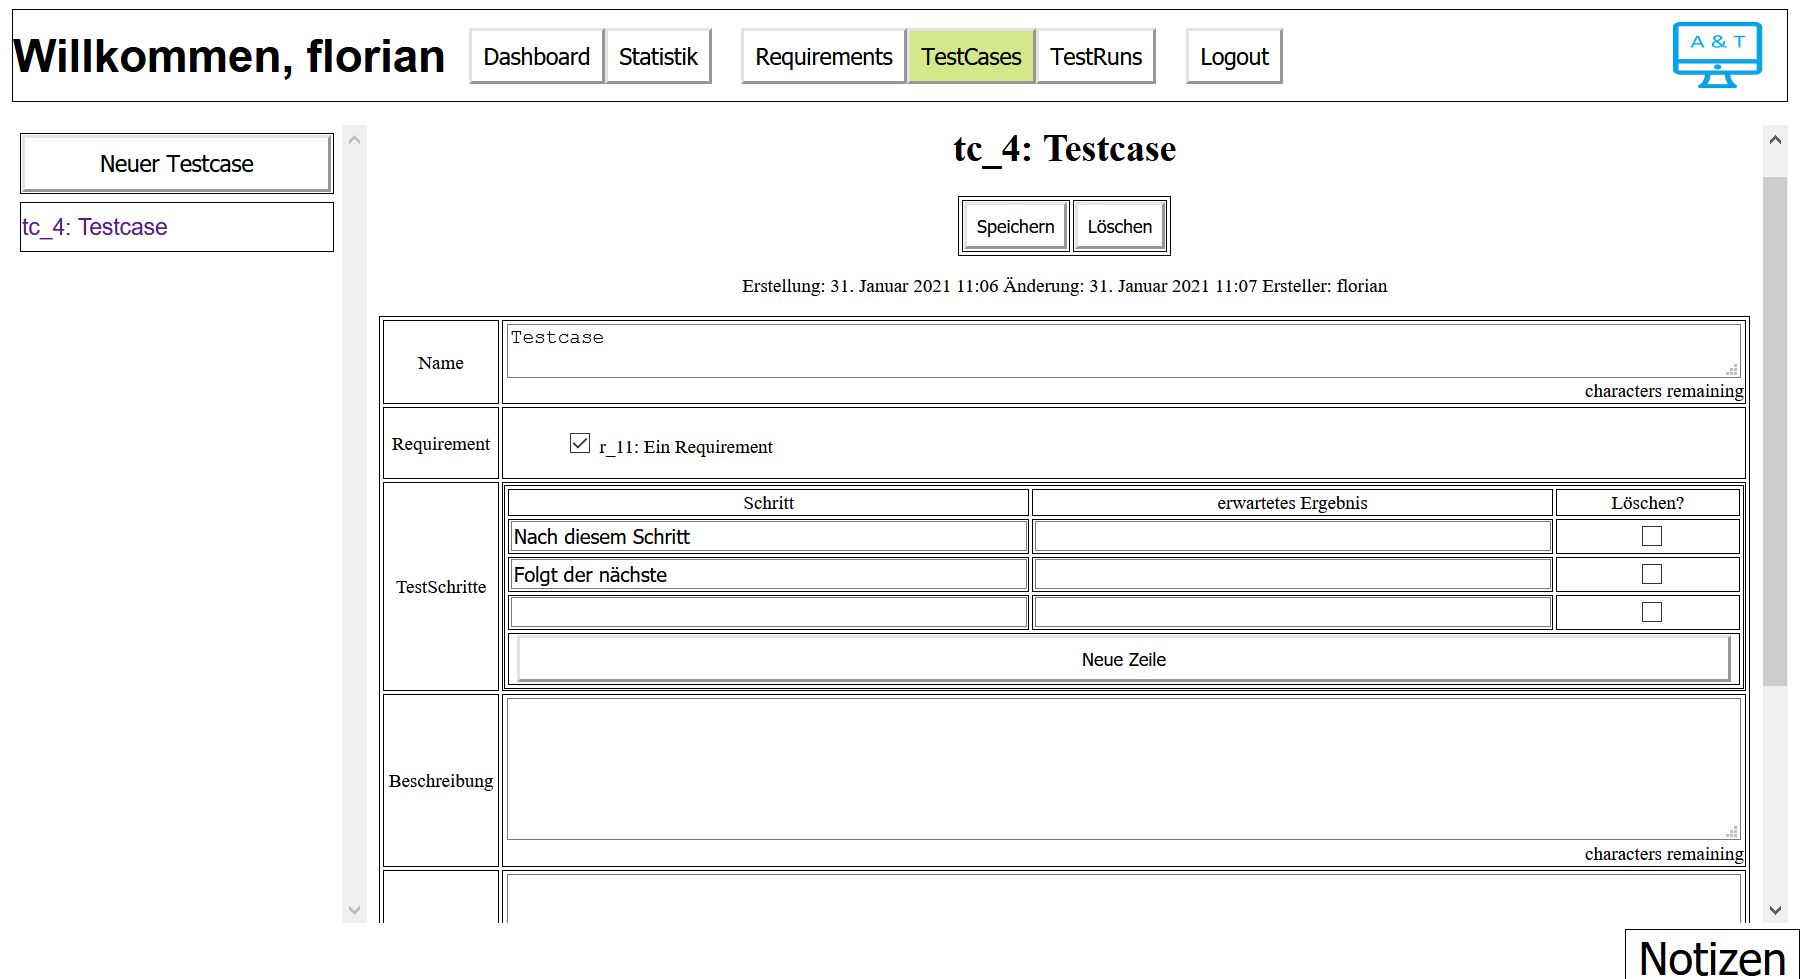
\includegraphics[width=1\textwidth]{testcase.png}
  \caption{Das Bearbeiten eines Testcase, eigene Darstellung}
  \label{f:testcase}
\end{figure}




Die Software \textit{"`Anforderungen und Testen"'} bietet verschiedene Features an, um das \textit{Anforderungs- und Testmanagement} zu unterstützen. Es können \textit{Requirements}, \textit{Testcases} und \textit{Testruns} erstellt werden. Dazu können die gewünschten Felder aus den Anforderungen A60, A70 und A80 mit Werten befüllt werden. In der Abbildung \ref{f:testcase} ist beispielsweise die Bearbeitungsseite der \textit{Testcases} dargestellt.



\begin{figure}[htpb]
  \centering
  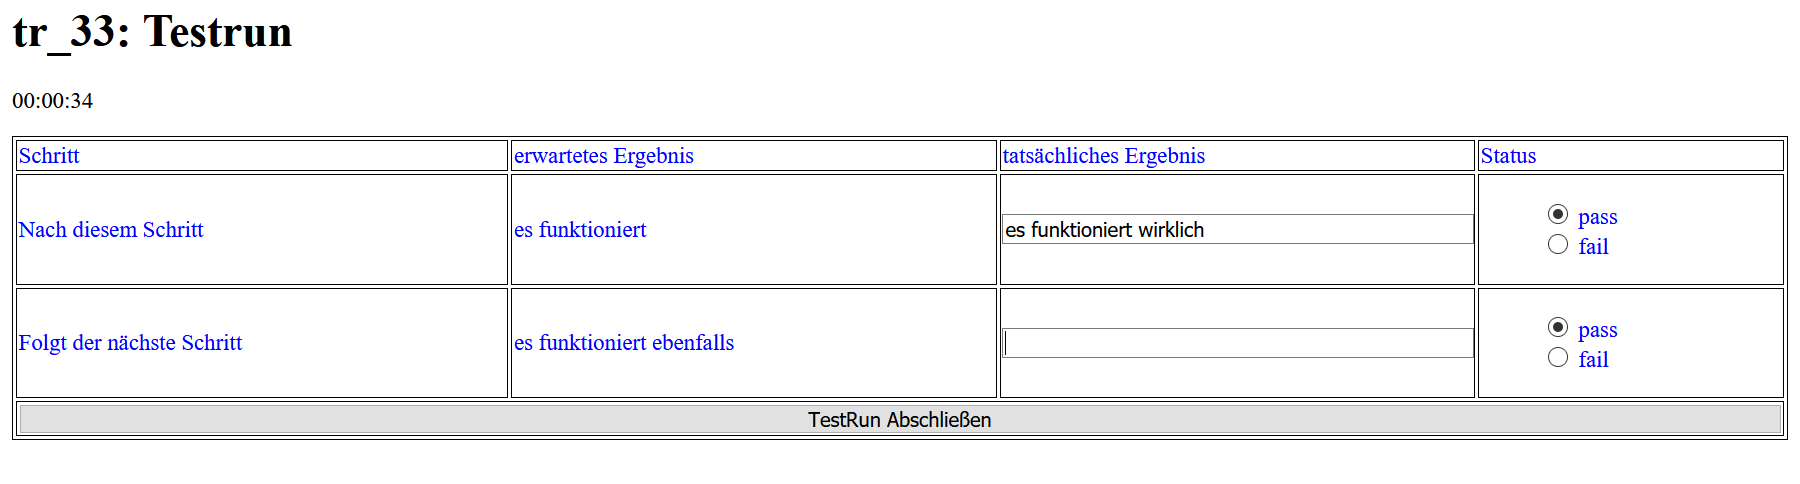
\includegraphics[width=1\textwidth]{testrun.png}
  \caption{Die Durchführung eines Testruns, eigene Darstellung}
  \label{f:testrun}
\end{figure}


\begin{listing}[htbp]
\begin{lstlisting}[
   basicstyle=\fontsize{9}{9}\selectfont\ttfamily
]
if all(item == list_mit_Ergebnissen[0] == 'p' for item in list_mit_Ergebnissen):
	testr_instance.testr_status = 'p'
else:
	testr_instance.testr_status = 'f'   
\end{lstlisting}
\caption{Der Generator Ausdruck}
\label{code:allsam}
\end{listing}



Daneben bietet die Software auch die wichtige Funktion, \textit{Testruns} nicht nur zu definieren, sondern diese auch durchzuführen. Die Durchführung ist in der Abbildung \ref{f:testrun} zu sehen. Dabei wird die Zeit, die gebraucht wird um ihn durchzuführen, gestoppt \cite{sotimer}. Erst wenn bei allen Testschritten der Status "`pass"' ausgewählt wurde, gilt dieser \textit{Testrun} als erfolgreich durchgeführt. Die Logik, die das prüft, ist im Listing \ref{code:allsam} dargestellt und wird als \textit{Generator-Ausdruck} realisiert. Die Variable \verb|list_mit_Ergebnissen| enthält dabei den Status aller \textit{Testschritte} als Liste \cite{soallsame}. Bevor der Nutzer die Seite verlässt, zum Beispiel um den \textit{Testrun} abzuschließen, wird er um eine Bestätigung der Aktion gebeten. Dadurch soll verhindert werden, dass der Nutzer aus Versehen den \textit{Testrun} frühzeitig beendet \cite{confirm}.



\begin{figure}[htpb]
  \centering
  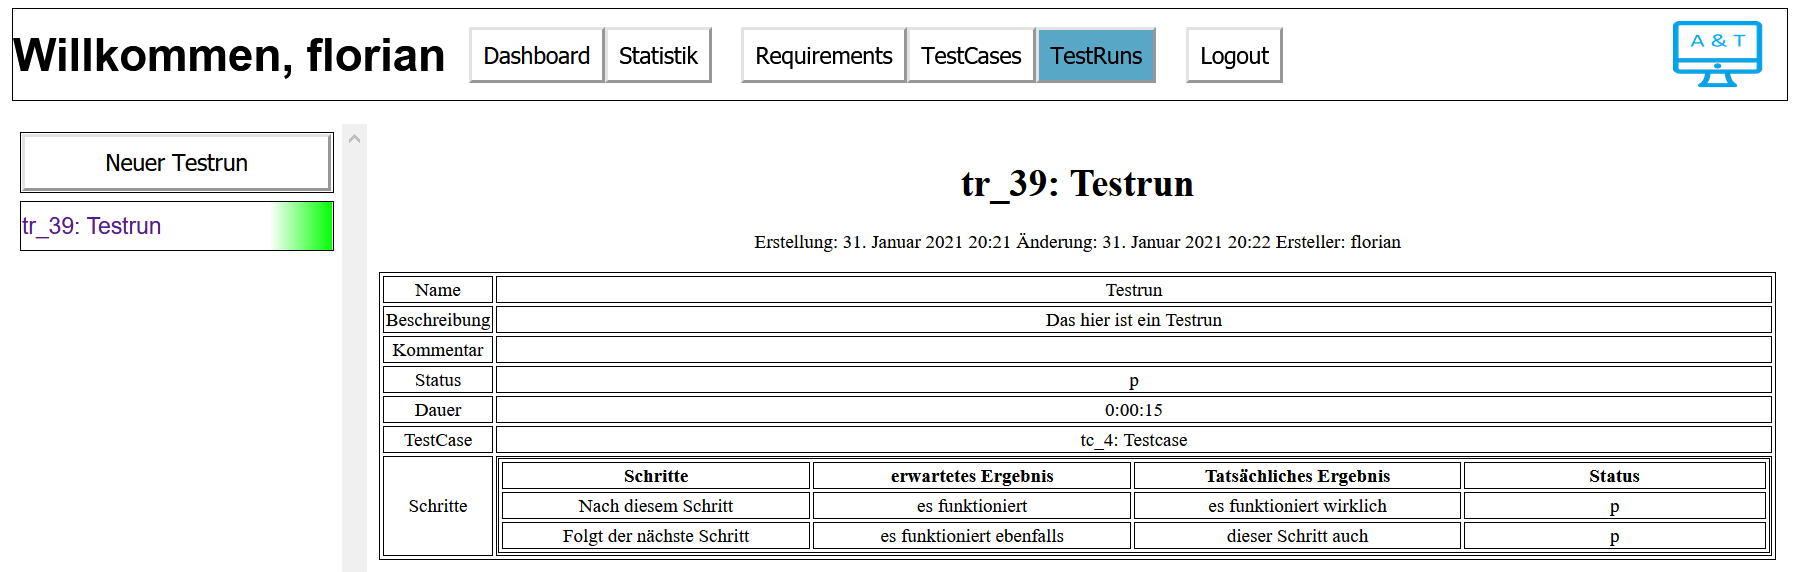
\includegraphics[width=1\textwidth]{testrunab.png}
  \caption{Die Anzeige bei einem abgeschlossenen Testrun, eigene Darstellung}
  \label{f:testrunab}
\end{figure}


Nachdem ein \textit{Testrun} durchgeführt wurde, ist er nicht mehr editierbar. Stattdessen zeigt er, wie in Abbildung \ref{f:testrunab} gezeigt, den getesteten \textit{Testcase} mit seinen Schritten und Ergebnissen an. Eine farbige Markierung an der linken Seite in der Listenübersicht zeigt ebenfalls an, ob der \textit{Testrun} erfolgreich war oder nicht.




Während der \textit{Login} und \textit{Logout} auf der von \textit{Django} vorgegebenen Authentifizierung basiert \cite{mozillatuto10}, musste der \textit{Signup} Prozess extra eingebracht werden \cite{signup}. Der Nutzen davon soll sein, dass sich die Studenten eigene Accounts anlegen können mit einem Benutzernamen, Passwort und einer Gruppennummer. Dadurch muss der Admin beziehungsweise der Professor nicht für jeden Student einen eigenen Account anlegen.

 
 



\chapter{Usability Test} \label{chap:use}
Damit ein \textit{Usabilitytest} durchgeführt werden konnte, wurde das Tool \textit{"`Anforderungen und Testen"'} auf der Webseite \textit{Heroku} hochgeladen und steht unter dem Link \url{https://anforderungen-und-testen.herokuapp.com/aut/} zum Testen bereit \cite{heroku}.

Der Inhalt des \textit{Usabilitytests} bestand darin, jeweils ein \textit{Requirement}, \textit{Testcase} und \textit{Testrun} zu erstellen. Dazu wurden Beispieldaten in einer Anleitung angegeben. Darüber hinaus sollte ein \textit{Testrun} durchgeführt werden, bevor zuletzt die Statistik Seite überprüft werden sollte.

Daraus folgten verschiedene Rückmeldungen, die zu einer Verbesserung der Software führen sollten. Der Notizen-Button sollte größer gemacht werden, damit er auffälliger wird. Die Seite auf die der \textit{Testrun} durchgeführt wird, sollte auch überarbeitet werden und die einzutragenden Felder ersichtlicher machen. Eine Tabelle sollte hier verwendet werden, um das zu erreichen.


Nachdem ein Element abgespeichert wurde, war nur sofort ersichtlich, dass etwas gespeichert wurde, wenn sich der Name verändert hat. Basierend auf diesem Feedback wurde in \textit{HTML} eine \textit{Snackbar} beziehungsweise ein \textit{Toast} realisiert. Dadurch bekommen die Nutzer ein Feedback, wenn der "`Speichern"'-Button gedrückt wird \cite{snack}.

Die Begrenzung der erlaubten Zeichen in den Eingabefeldern wurde ebenfalls überdacht, da die Nutzer nicht genug Platz hatten, um die Texte einzugeben. Die Länge der Felder wurde somit vergrößert.

Auf dem \textit{Dashboard} sollte es eine bessere Unterscheidung geben zwischen anklickbaren Buttons und der Tabelle. Durch ein neues Design der Buttons stechen diese nun besser hervor.

Eine weitere Rückmeldung war, das die Gebrauchsanleitung in irgendeiner Form der Software beiliegen sollte, um vor allem die Farben zu erklären. Dazu wurden auf den Seiten der \textit{Requirements}, \textit{Testcases} und \textit{Testruns} Erklärungen geschrieben, die angezeigt werden, falls kein Element ausgewählt ist.




\chapter{Fazit} \label{chap:fazit}

Die Kategorie, die als Attribut bei den \textit{Requirements} gefordert wurde, wurde in dieser Version nicht implementiert. In einer zweiten Version könnten die Kategorien ausgebaut werden, um so die verschiedenen Arten von Anforderungen, wie in Kapitel \ref{s:anfundtest} aufgelistet, zu unterscheiden. Der Nutzer könnte ebenfalls in der Lage sein eigene Kategorien zu definieren. Dann würde sich anbieten eine Suche oder einen Filter zu implementieren. Da diese Features eher ablenken würden, war es vorzuziehen, sich diese für eine zweite Version zu merken.


Eine Überarbeitung des \textit{Dashboards} in Form einer Verschönerung könnte ebenfalls sinnvoll sein, um die Informationen schneller vermitteln zu können. Es könnten Diagramme und andere Darstellungsformen, wie die vorgestellten Tools in Kapitel \ref{chap:Tools} sie benutzen, verwendet werden.
 
 
Abschließend kann zusammengefasst werden, dass die gestellten Anforderungen durch die Software \textit{"`Anforderungen und Testen"'} erfüllt werden und die Erstellung eines leichtgewichtigen \textit{Softwaretools} für das \textit{Anforderungs- und Testmanagement} im \textit{Softwareentwicklungsumfeld} somit erfolgreich abschlossen werden konnte.



\newpage

% Listen wenn überhaupt ans Ende und nicht an den Anfang.
% Meist ist das aber unnötig.
% \listoffigures % Liste der Abbildungen 
% \listoftables % Liste der Tabellen
% \newpage

\bibliographystyle{plain} % Literaturverzeichnis
\begin{btSect}{thesis} % mit bibtopic Quellen trennen
\section*{Literaturverzeichnis}
\btPrintCited
\end{btSect}
\begin{btSect}{online}
\section*{Online-Quellen}
\btPrintCited
\end{btSect}
% dann mit "
% thesis1" und "bibtex thesis2" arbeiten

\end{document}
;;; Local Variables:
;;; ispell-local-dictionary: "de_DE-neu"
;;; End:
